%%% ======= Beamer ======
\documentclass[usenames,dvipsnames,t]{beamer}
% \documentclass[usenames,dvipsnames, handout]{beamer}
\beamertemplatenavigationsymbolsempty % remove toolbar at the bottom of slides
\usepackage{appendixnumberbeamer} % for appendix
\usetheme{Madrid}
\usecolortheme{default}
\useinnertheme{circles}

\setbeamercolor{author in head/foot}{bg=blue!10, fg=blue}
\setbeamercolor{title in head/foot}{bg=blue!10, fg=blue}
\setbeamercolor{date in head/foot}{bg=blue!10, fg=blue}

\makeatletter
\setbeamertemplate{footline}{
  \leavevmode%
  \hbox{%
  \begin{beamercolorbox}[wd=.333333\paperwidth,ht=2.25ex,dp=1ex,center]{author in head/foot}%
    \usebeamerfont{author in head/foot}\insertshortauthor\expandafter\ifblank\expandafter{\beamer@shortinstitute}{}{~~(\insertshortinstitute)}
  \end{beamercolorbox}%
  \begin{beamercolorbox}[wd=.333333\paperwidth,ht=2.25ex,dp=1ex,center]{title in head/foot}%
    \usebeamerfont{title in head/foot}\insertshorttitle
  \end{beamercolorbox}%
  \begin{beamercolorbox}[wd=.333333\paperwidth,ht=2.25ex,dp=1ex,right]{date in head/foot}%
    \usebeamerfont{date in head/foot}\insertshortdate{}\hspace*{2em}
    \insertframenumber{}%
%     / \inserttotalframenumber
    \hspace*{2ex} 
  \end{beamercolorbox}}%
  \vskip0pt%
}
\makeatother

\colorlet{beamer@blendedblue}{blue!70} % change color theme

\usepackage[style=numeric-comp,sorting=none,backend=biber]{biblatex}%<- specify style
\addbibresource{references.bib}%<- specify bib file

\usepackage{svg}


% For appendix
\newcommand{\backupbegin}{
   \newcounter{framenumberappendix}
   \setcounter{framenumberappendix}{\value{framenumber}}
}
\newcommand{\backupend}{
   \addtocounter{framenumberappendix}{-\value{framenumber}}
   \addtocounter{framenumber}{\value{framenumberappendix}} 
}

\setbeamertemplate{bibliography item}{\insertbiblabel} % improved references



% Other preamble stuff:
\usepackage{preamble}

%%% Uncomment for another color palette
% \definecolor{Logo1}{rgb}{0.0, 0, 0.7}
% \definecolor{Logo2}{rgb}{2.55, 2.55, 2.55}

% \setbeamercolor*{palette primary}{bg=Logo1, fg=white}
% \setbeamercolor*{palette secondary}{bg=Logo2, fg=white}
% \setbeamercolor*{palette tertiary}{bg=white, fg=Logo1}
% \setbeamercolor*{palette quaternary}{bg=white,fg=white}
% \setbeamercolor{structure}{fg=Logo1} % itemize, enumerate, etc
% \setbeamercolor{section in toc}{fg=Logo1} % TOC sections

% For figures
\usepackage{import}
\usepackage{xifthen}
\usepackage{pdfpages}
\usepackage{transparent}
\usepackage{mdframed}
\usepackage{subcaption}

\setbeamertemplate{caption}[numbered]



% --- Inkscape figures:
\newcommand{\incfig}[2][0.75\textwidth]{%
    \def\svgwidth{\columnwidth}
    \resizebox{#1}{!}{\import{Inkscape figs/}{#2.pdf_tex}}
}

% --- Height of frame
\newlength{\myheight}
\setlength{\myheight}{7cm}

\newlength\myheightfigureintext
\newlength\mydepthfigureintext
\settototalheight\myheightfigureintext{Xygp}
\settodepth\mydepthfigureintext{Xygp}
\setlength\fboxsep{0pt}


%------------------------------------------------------------
%This block of code defines the information to appear in the
%Title page
\title[\textsc{Jim} for BNS PE] %optional
{Accelerating parameter estimation of binary neutron star mergers with normalizing flows}

\author[Thibeau Wouters]{\small{\textbf{Thibeau Wouters}, Peter T.H. Pang, Tim Dietrich, Chris Van Den Broeck} \\ \vspace{7mm} email: \href{mailto:t.r.i.wouters@uu.nl}{t.r.i.wouters@uu.nl} \\ \vspace{7mm} \href{http://arxiv.org/abs/2404.11397}{arXiv:2404.11397}}

% \raisebox{-\mydepthfigureintext}{\fbox{
\includegraphics[height=\myheightfigureintext]{Figures/arxiv_logo_red_no_background.png}}}

\date{AIslands 2024}




%End of title page configuration block
%------------------------------------------------------------



%------------------------------------------------------------
%The next block of commands puts the table of contents at the 
%beginning of each section and highlights the current section:

\AtBeginSection[]
{
  \begin{frame}[plain, noframenumbering]
    \frametitle{Table of Contents}
    \tableofcontents[currentsection]
  \end{frame}
}


%------------------------------------------------------------


\begin{document}

{

\usebackgroundtemplate{\transparent{0.15}{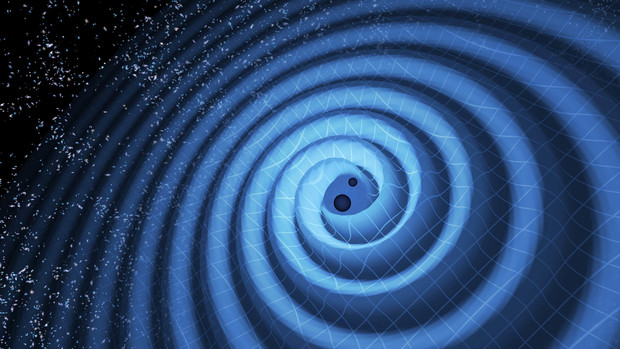
\includegraphics[width=\paperwidth,height=\paperheight]{Figures/GW-2.jpeg}}}

\begin{frame}[plain]
\titlepage

\begin{columns}
  \column{0.35\textwidth}
  \begin{figure}
    \centering
    \vspace{1.5mm}
    
\includegraphics[width=0.75\linewidth]{Figures/utrecht-university.png}
  \end{figure}
  \column{0.35\textwidth}
  \begin{figure}
    \centering
    
\includegraphics[width=0.75\linewidth]{Figures/Nikhef_logo-transparent.png}
  \end{figure}
\end{columns}


%%% as subfigures
% \begin{figure}
%   \centering
%   \begin{subfigure}[b]{0.475\textwidth}
%     \centering
%     
\includegraphics[width=0.6\textwidth]{Figures/utrecht-university.png}
%   \end{subfigure}
%   \caption*{}
%   \hfill
%   \begin{subfigure}[b]{0.475\textwidth}
%     \centering
%     
\includegraphics[width=0.6\textwidth]{Figures/Nikhef_logo-transparent.png}
%   \end{subfigure}
%   \caption*{}
%   % \caption*{}
% \end{figure}

\end{frame}
}

% %The next statement creates the title page.
% \frame[plain]{\titlepage



% }


%---------------------------------------------------------
%This block of code is for the table of contents after
%the title page
% \begin{frame}[plain, noframenumbering]
% \frametitle{Table of Contents}
% \tableofcontents
% \end{frame}
%---------------------------------------------------------


\section{Introduction}

\begin{frame}{Parameter estimation}

\def\x{3mm}
\def\y{2mm}

Parameter estimation (PE): get \red{posterior} of GW parameters $\theta$ % from data $d$
\begin{equation*}
    \red{p(\theta | d)} = \frac{p(d | \theta) p(\theta)}{p(d)} = \frac{\text{likelihood} \times \text{prior}}{\text{evidence}}
\end{equation*}

\vspace{1mm}

% \begin{equation}\label{eq: likelihood function}
%   \log p(d|\theta) \propto\left\langle d - h(\boldsymbol{\theta}), d - h(\boldsymbol{\theta}) \right\rangle
% \end{equation}

\begin{tcolorbox}[colback=blue!10, boxrule=0pt]
  \textbf{Problem:} Markov Chain Monte Carlo (MCMC): computationally expensive for binary neutron stars (BNS)
\end{tcolorbox}


\vspace{-1mm}

\begin{figure}
  \centering
  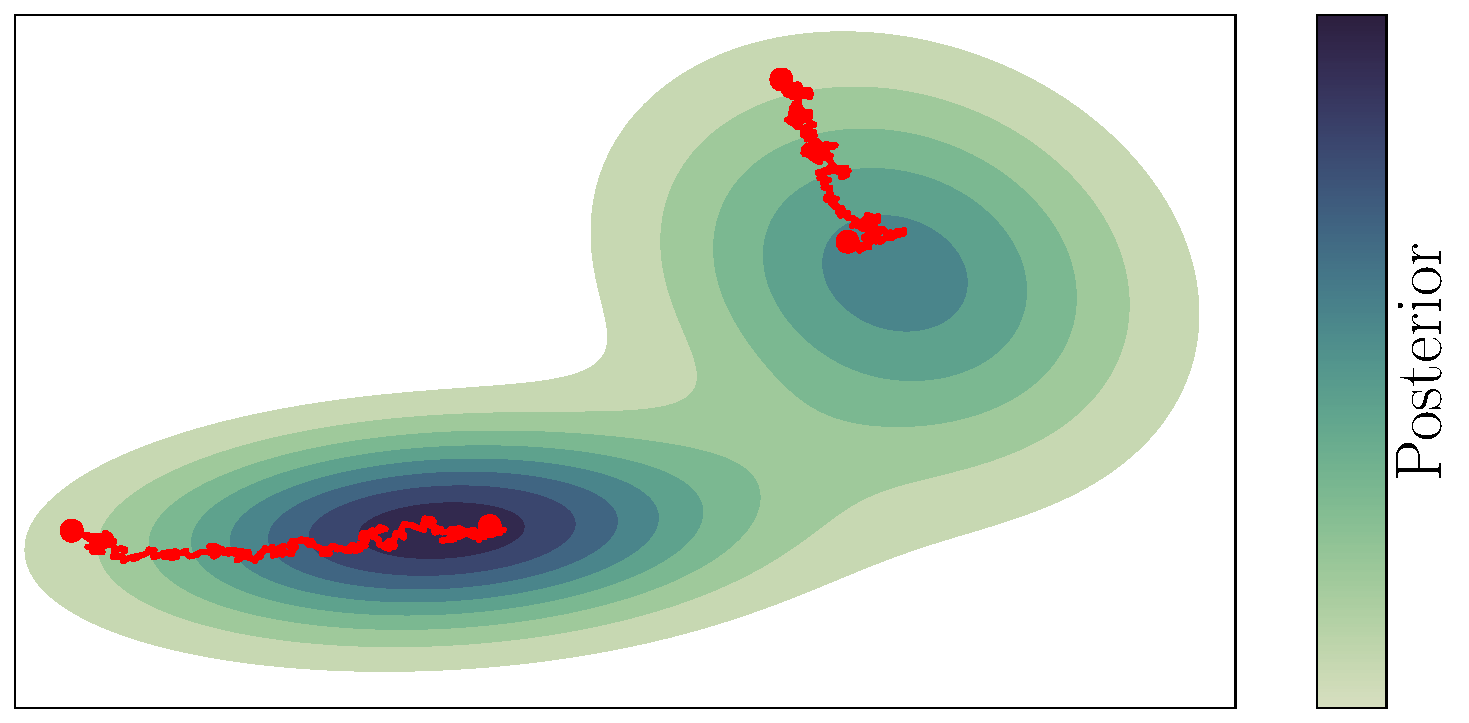
\includegraphics[width=0.65\textwidth]{Figures/mixture_of_gaussians_projection_no_title_colorbar.pdf}
  \caption*{}
\end{figure}

\end{frame}


\begin{frame}{Overview}

  \def\x{4mm}
  \def\y{4mm}

\textsc{Jim}: fast parameter estimation of GW signals with \textsc{jax}

\vspace{\y}
\begin{itemize}
  \item MCMC sampler: \textsc{flowMC}

  \vspace{\y}

  \item Waveforms: \textsc{ripple}
\end{itemize}
% \vspace{\x}
% \begin{enumerate}
%   \item \textsc{flowMC}: Normalizing flow-enhanced, gradient-based MCMC
  
%   \vspace{\x}

%   \item \textsc{ripple}: Automatically-differentiable (AD) GW
  
%   \vspace{\x}

%   \item \textcolor{gray}{Relative binning likelihood}
% \end{enumerate}

\vspace{\x}

\incfig[\textwidth]{jim_flowMC_ripple}
  

\end{frame}


\section{Methods}

% \begin{frame}{\textsc{jax}}

%   \def\x{4mm}

%   \begin{tcolorbox}[colback=blue!10, boxrule=0pt]
%     What are the benefits of \textsc{jax} for MCMC?
%   \end{tcolorbox}

% \vspace{3mm}

% \begin{columns}
%   \column{0.75\textwidth}
%   \begin{enumerate}
%     \item Automatic differentiation (AD)
    
%     \vspace{\x}

%     \item Just-in-time (JIT) compilation
    
%     \vspace{\x}
    
%     \item GPU acceleration
    
%     \vspace{\x}
    
%     \item Parallelization
    
%     % \vspace{\x}
    
%     % \item Vectorization
    
%     % \vspace{\x}
    
%     % \item Interoperability with \texttt{numpy}
%   \end{enumerate}
%   \column{0.20\textwidth}
%   \begin{figure}
%     % \centering
%     
\includegraphics[width=\textwidth]{Figures/jax.png}
%   \end{figure}
% \end{columns}
  
% \end{frame}

\begin{frame}{Normalizing flows}

  \def\x{3mm}
  \def\y{7mm}
  
  
  % \begin{enumerate}
  %   \setcounter{enumi}{1}
  %   \item \textbf{Train normalizing flow:}
  % \end{enumerate}
  
  % \vspace{\x}
  
  \begin{itemize}
    % \item \blue{Latent space}: easy to sample (e.g. Gaussian)
    
    % \vspace{\x}
  
    % \item \red{Parameter space}: complicated distribution
    
    % \vspace{\x}

    \item Generative machine learning model

    \vspace{\x}

    \item Learn mapping between \blue{latent} and \red{parameter} space

    \vspace{\x}
    
    \item Enable approximate sampling from complicated distributions

    \vspace{\x}
    
    \item Training data: MCMC samples
  \end{itemize}
  
  \vspace{\y}
    
  \incfig[\textwidth]{NF}
  
\end{frame}

\begin{frame}{\textsc{flowMC}}

  \def\x{3mm}
  \def\y{4mm}
  \def\z{2mm}
  
  \textsc{flowMC}: normalizing-flow (NF) enhanced MCMC sampling
  \vspace{\y}
  \begin{enumerate}
    \item Gradient-based sampler (local sampler)
  
    \vspace{\y}

    \item Train NF with samples from local sampler
  
    \vspace{\y}

    \item Sample normalizing flow (global sampler)
  \end{enumerate}
  
  \vspace{\z}
  
  \begin{figure}
    \centering
    \incfig[\textwidth]{flowMCOverview2}
  \end{figure}
\end{frame}

% \begin{frame}{\textsc{flowMC} -- local sampling}

%   \def\x{2mm}

%   \begin{enumerate}
%     \item \textbf{Local sampling}: Metropolis-adjusted Langevin algorithm (MALA)
    
%     \vspace{3mm}
    
%     \begin{itemize}
%       \item Proposal \red{$y$}: Langevin diffusion
%       \begin{equation*}
%         \red{y} = x + \frac{\epsilon^2}{2} \nabla \log p(x) + \epsilon \xi
%       \end{equation*}

%       \vspace{\x}
  
%       \item Gradient with \textsc{jax}
      
%       \vspace{\x}
      
%       \item Metropolis-Hastings acceptance step
%     \end{itemize}
    
%   \end{enumerate}
  
%   % \incfig[\textwidth]{MALA}
%   \begin{figure}
%     \centering
%     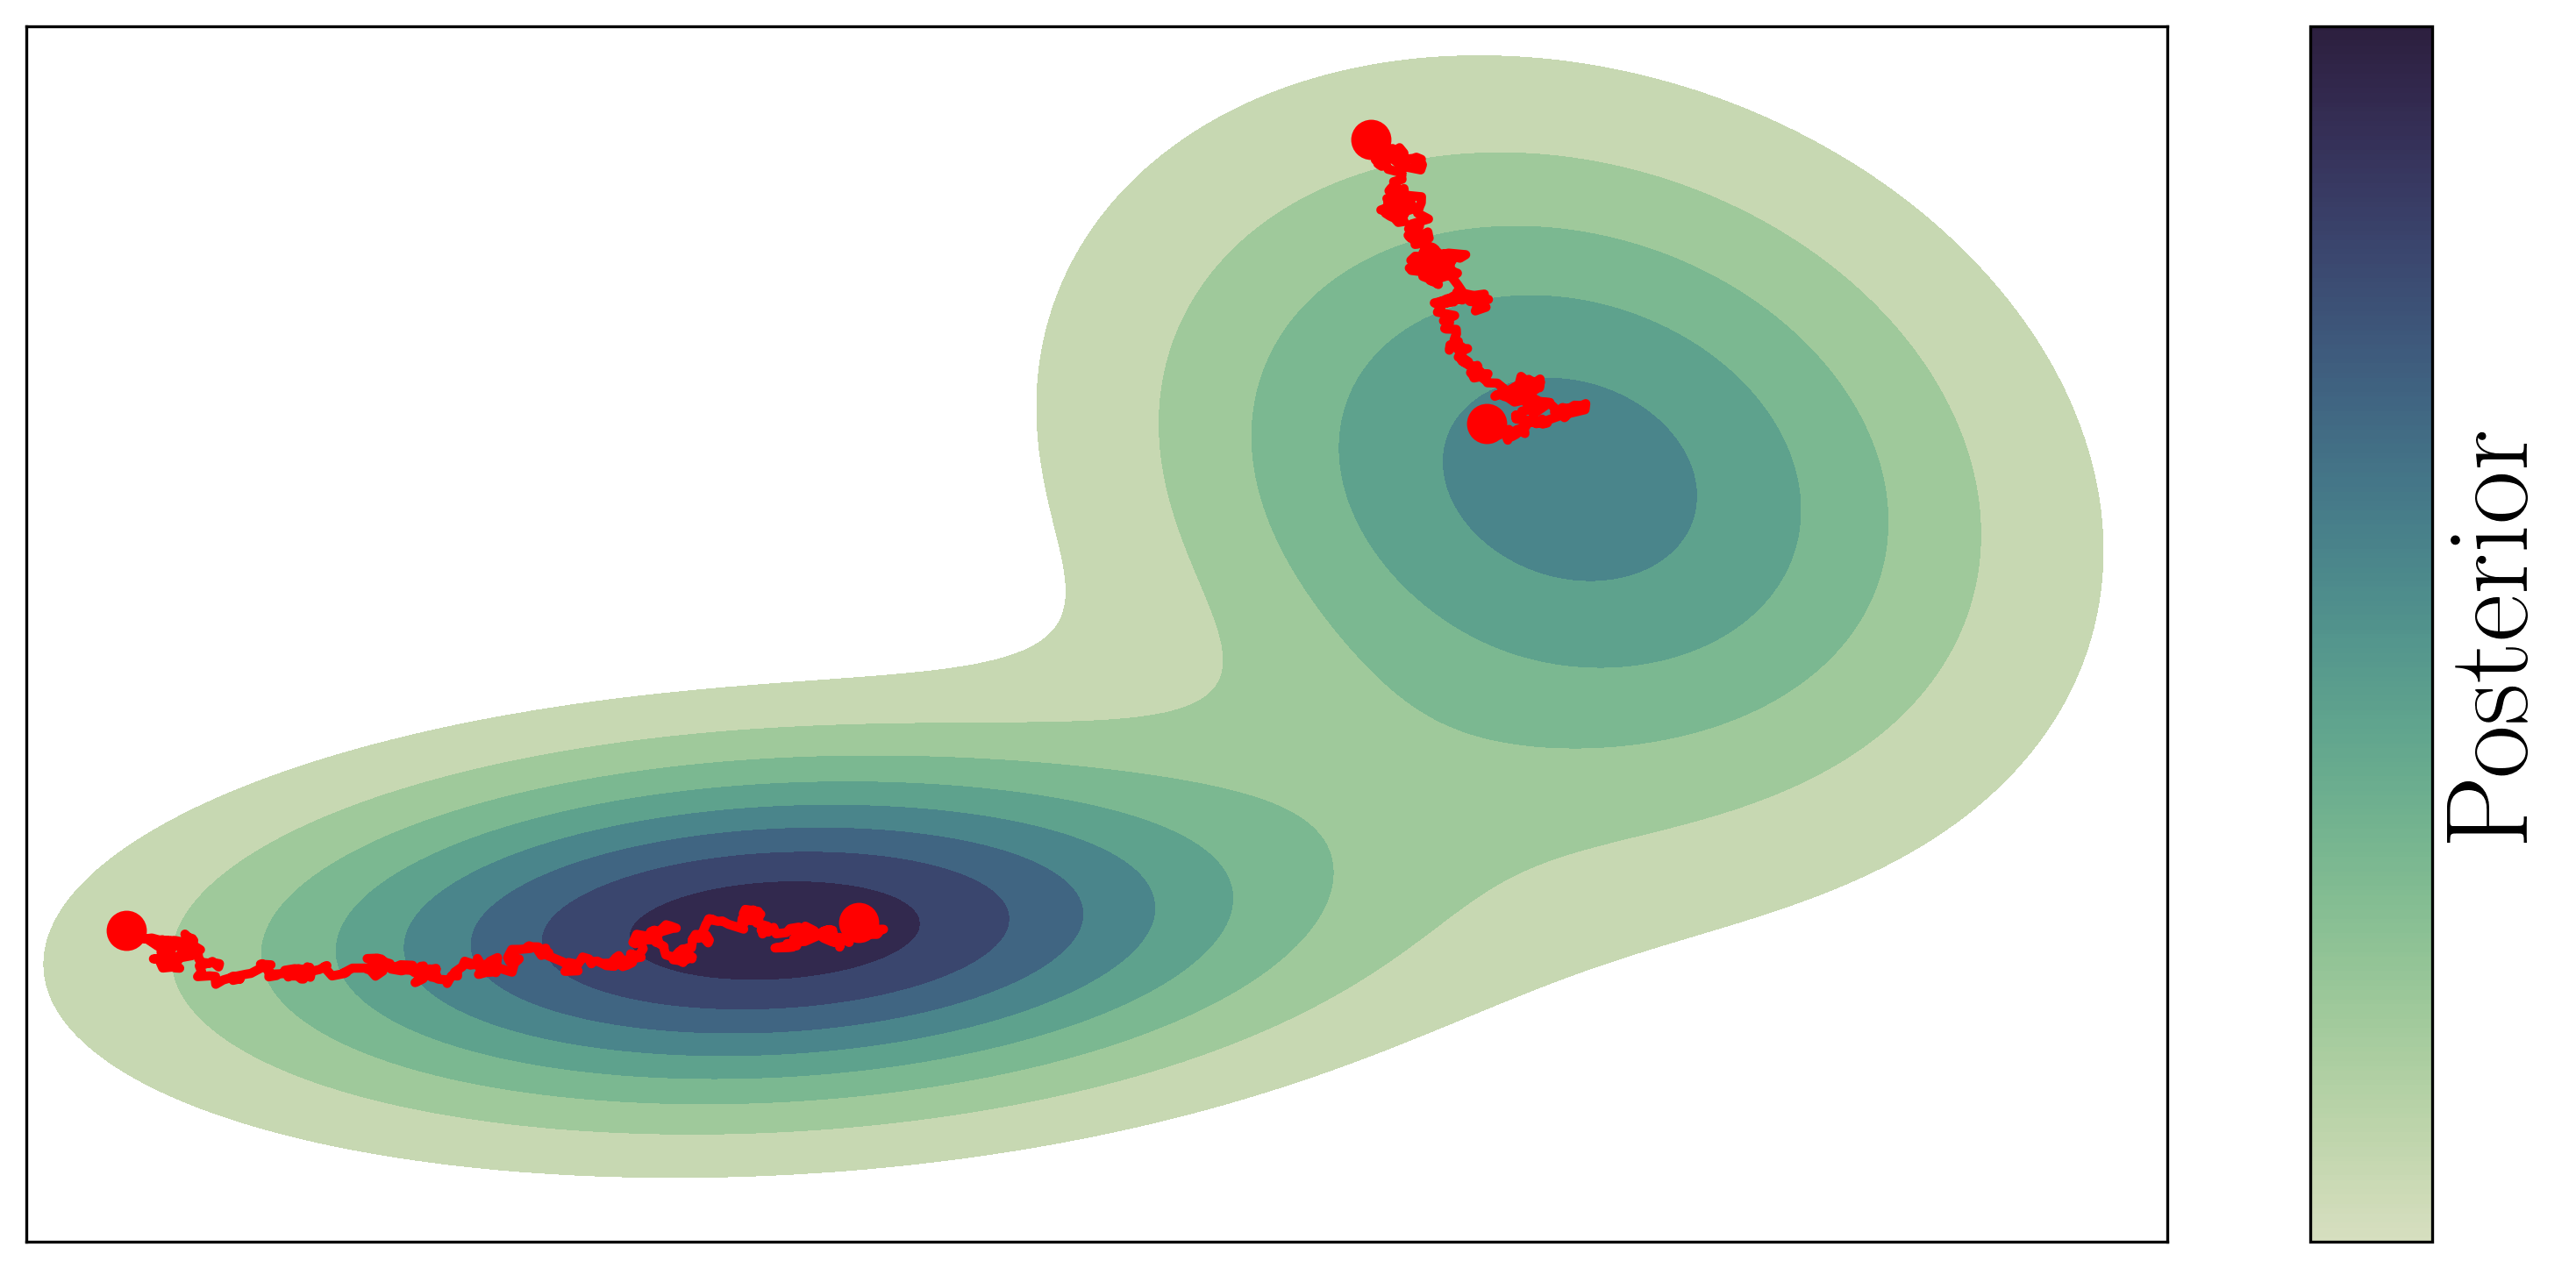
\includegraphics[scale = 0.3]{Figures/mixture_of_gaussians_projection_no_title_colorbar.png}
%   \end{figure}
  
%   \end{frame}



% \begin{frame}{\textsc{flowMC} -- global sampling}

%   \def\x{3mm}
%   \def\y{2mm}

%   \begin{enumerate}
%     \setcounter{enumi}{2}
%     \item \textbf{Global sampling}
%   \end{enumerate}

%   \vspace{\x}

%   \begin{itemize}
%     \item Global proposal by sampling from NF
    
%     \vspace{\y}
    
%     \item Metropolis-Hastings acceptance step
%   \end{itemize}

%   % \vspace{8mm}
  
%   \begin{figure}
%     \centering
%     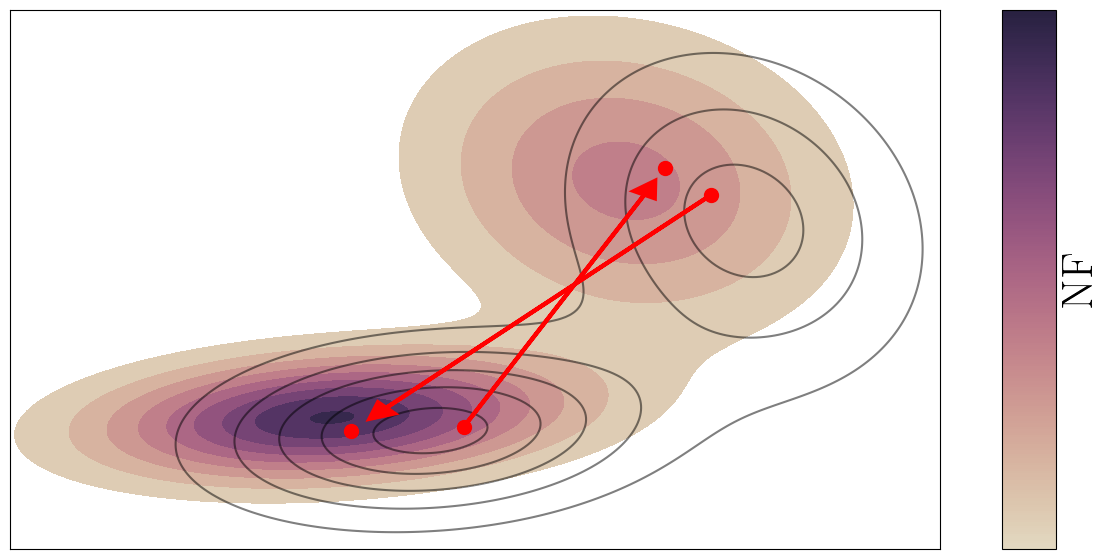
\includegraphics[width = 0.75\textwidth]{Figures/mixture_of_gaussians_projection_with_NF.png}
%   \end{figure}

% \end{frame}

% \begin{frame}{\textsc{flowMC} -- recap}

%   \def\x{3mm}
%   \def\y{3mm}
%   \def\z{-2mm}
  
%   \textsc{flowMC}: normalizing-flow (NF) enhanced MCMC sampling
%   \vspace{\y}

%   \begin{itemize}
%     \item Integrate with GW likelihood $\rightarrow$ \textsc{Jim}
    
%     \vspace{\y}
    
%     \item Stop training NF when Metropolis-Hastings acceptance is high
    
%     \vspace{\y}
    
%     \item Freeze weights, produce final samples
%   \end{itemize}
  
%   \begin{figure}
%     \centering
%     \incfig[\textwidth]{flowMCOverview2}
%   \end{figure}
% \end{frame}
  

\section{Results}

\begin{frame}{Results}

  \def\x{3mm}
  \def\y{1mm}

  \begin{itemize}
    % \item Implemented \texttt{TaylorF2}, \texttt{IMRPhenomD\_NRTidalv2} in \textsc{ripple}
    
    % \vspace{\x}

    % \item Robustness: injection campaign
    
    % \vspace{\x}

    % \item Analyzed injections \& 2 BNS events (posteriors: figures~\ref{fig: GW170817 TaylorF2},~\ref{fig: GW170817 NRTidalv2},~\ref{fig: GW190425 TaylorF2},~\ref{fig: GW190425 NRTidalv2})
    
    % \vspace{\x}
    
    \item Waveforms: \texttt{TaylorF2} (\texttt{TF2}), \texttt{IMRPhenomD\_NRTidalv2} (\texttt{NRTv2})

    \vspace{\x}

    \item<1> \textsc{Jim} wall time: (i) computing reference parameters for relative binning, (ii) training NF, (iii) sampling
  \end{itemize}

  \vspace{1mm}

  \scriptsize
  \onslide<1>{
  \begin{table}
    \centering
    \renewcommand{\arraystretch}{1.5}
    \begin{tabular}{ l l c c c c}
      \hline\hline
 Event & Waveform & \textsc{Jim} & \textsc{pBilby} & \textsc{RB-Bilby} & \textsc{ROQ-Bilby}  \\
 & & \scriptsize{($1$ GPU)} & \scriptsize{($480$ cores)} & \scriptsize{($24$ cores)} & \scriptsize{($24$ cores)} \\
  \hline\hline
 \multirow{2}{*}{GW170817} & \texttt{TF2} & $(9.70 + 17.00)$ min & $\phantom{0}9.64$ h & $3.18$ h & -- \\
 & \texttt{NRTv2} & $(5.69 + 28.02)$ min & $10.99$ h & $4.68$ h & $1.65$ h \\ \hline
\multirow{2}{*}{GW190425}  & \texttt{TF2} & $(5.13 + 16.49)$ min & $\phantom{0}4.08$ h & $2.30$ h & -- \\ 
 & \texttt{NRTv2} & $(6.15 + 15.37)$ min & $\phantom{0}4.69$ h & $4.68$ h & $0.97$ h \\ \hline
\multirow{2}{*}{Injection} & \texttt{TF2} & $\phantom{(0.000 + } 24.76\phantom{)}$ min & -- & -- & -- \\
& \texttt{NRTv2} & $\phantom{(0.000 + } 18.02\phantom{)}$ min & -- & -- & -- \\
\hline\hline
\end{tabular}
\label{tab: runtimes table full}
\end{table}

\normalsize

\vspace{\y}

\scriptsize{(\textsc{pBilby} = \textsc{Parallel Bilby}, RB = relative binning, ROQ = reduced order quadrature)}
}
\end{frame}

% \begin{frame}{Results -- GW170817 \& GW190425}
%     \def\x{3mm}

%     \begin{columns}
%       \column{0.325\textwidth}
%       \begin{itemize}
%         \item Compare with \textsc{pBilby}

%         \vspace{\x}
        
%         \item Cornerplots: Figure~\ref{fig: GW170817 TaylorF2},~\ref{fig: GW170817 NRTidalv2},~\ref{fig: GW190425 TaylorF2},~\ref{fig: GW190425 NRTidalv2}

%         \vspace{\x}
  
%         \item Jensen-Shannon divergences: Table~\ref{tab: JS divergences events}
        
%         \vspace{\x}
%         \item GW170817, \texttt{TaylorF2}:
%       \end{itemize}


%       \column{0.675\textwidth}
%     \vspace{-15.5mm}
%     \begin{figure}
%     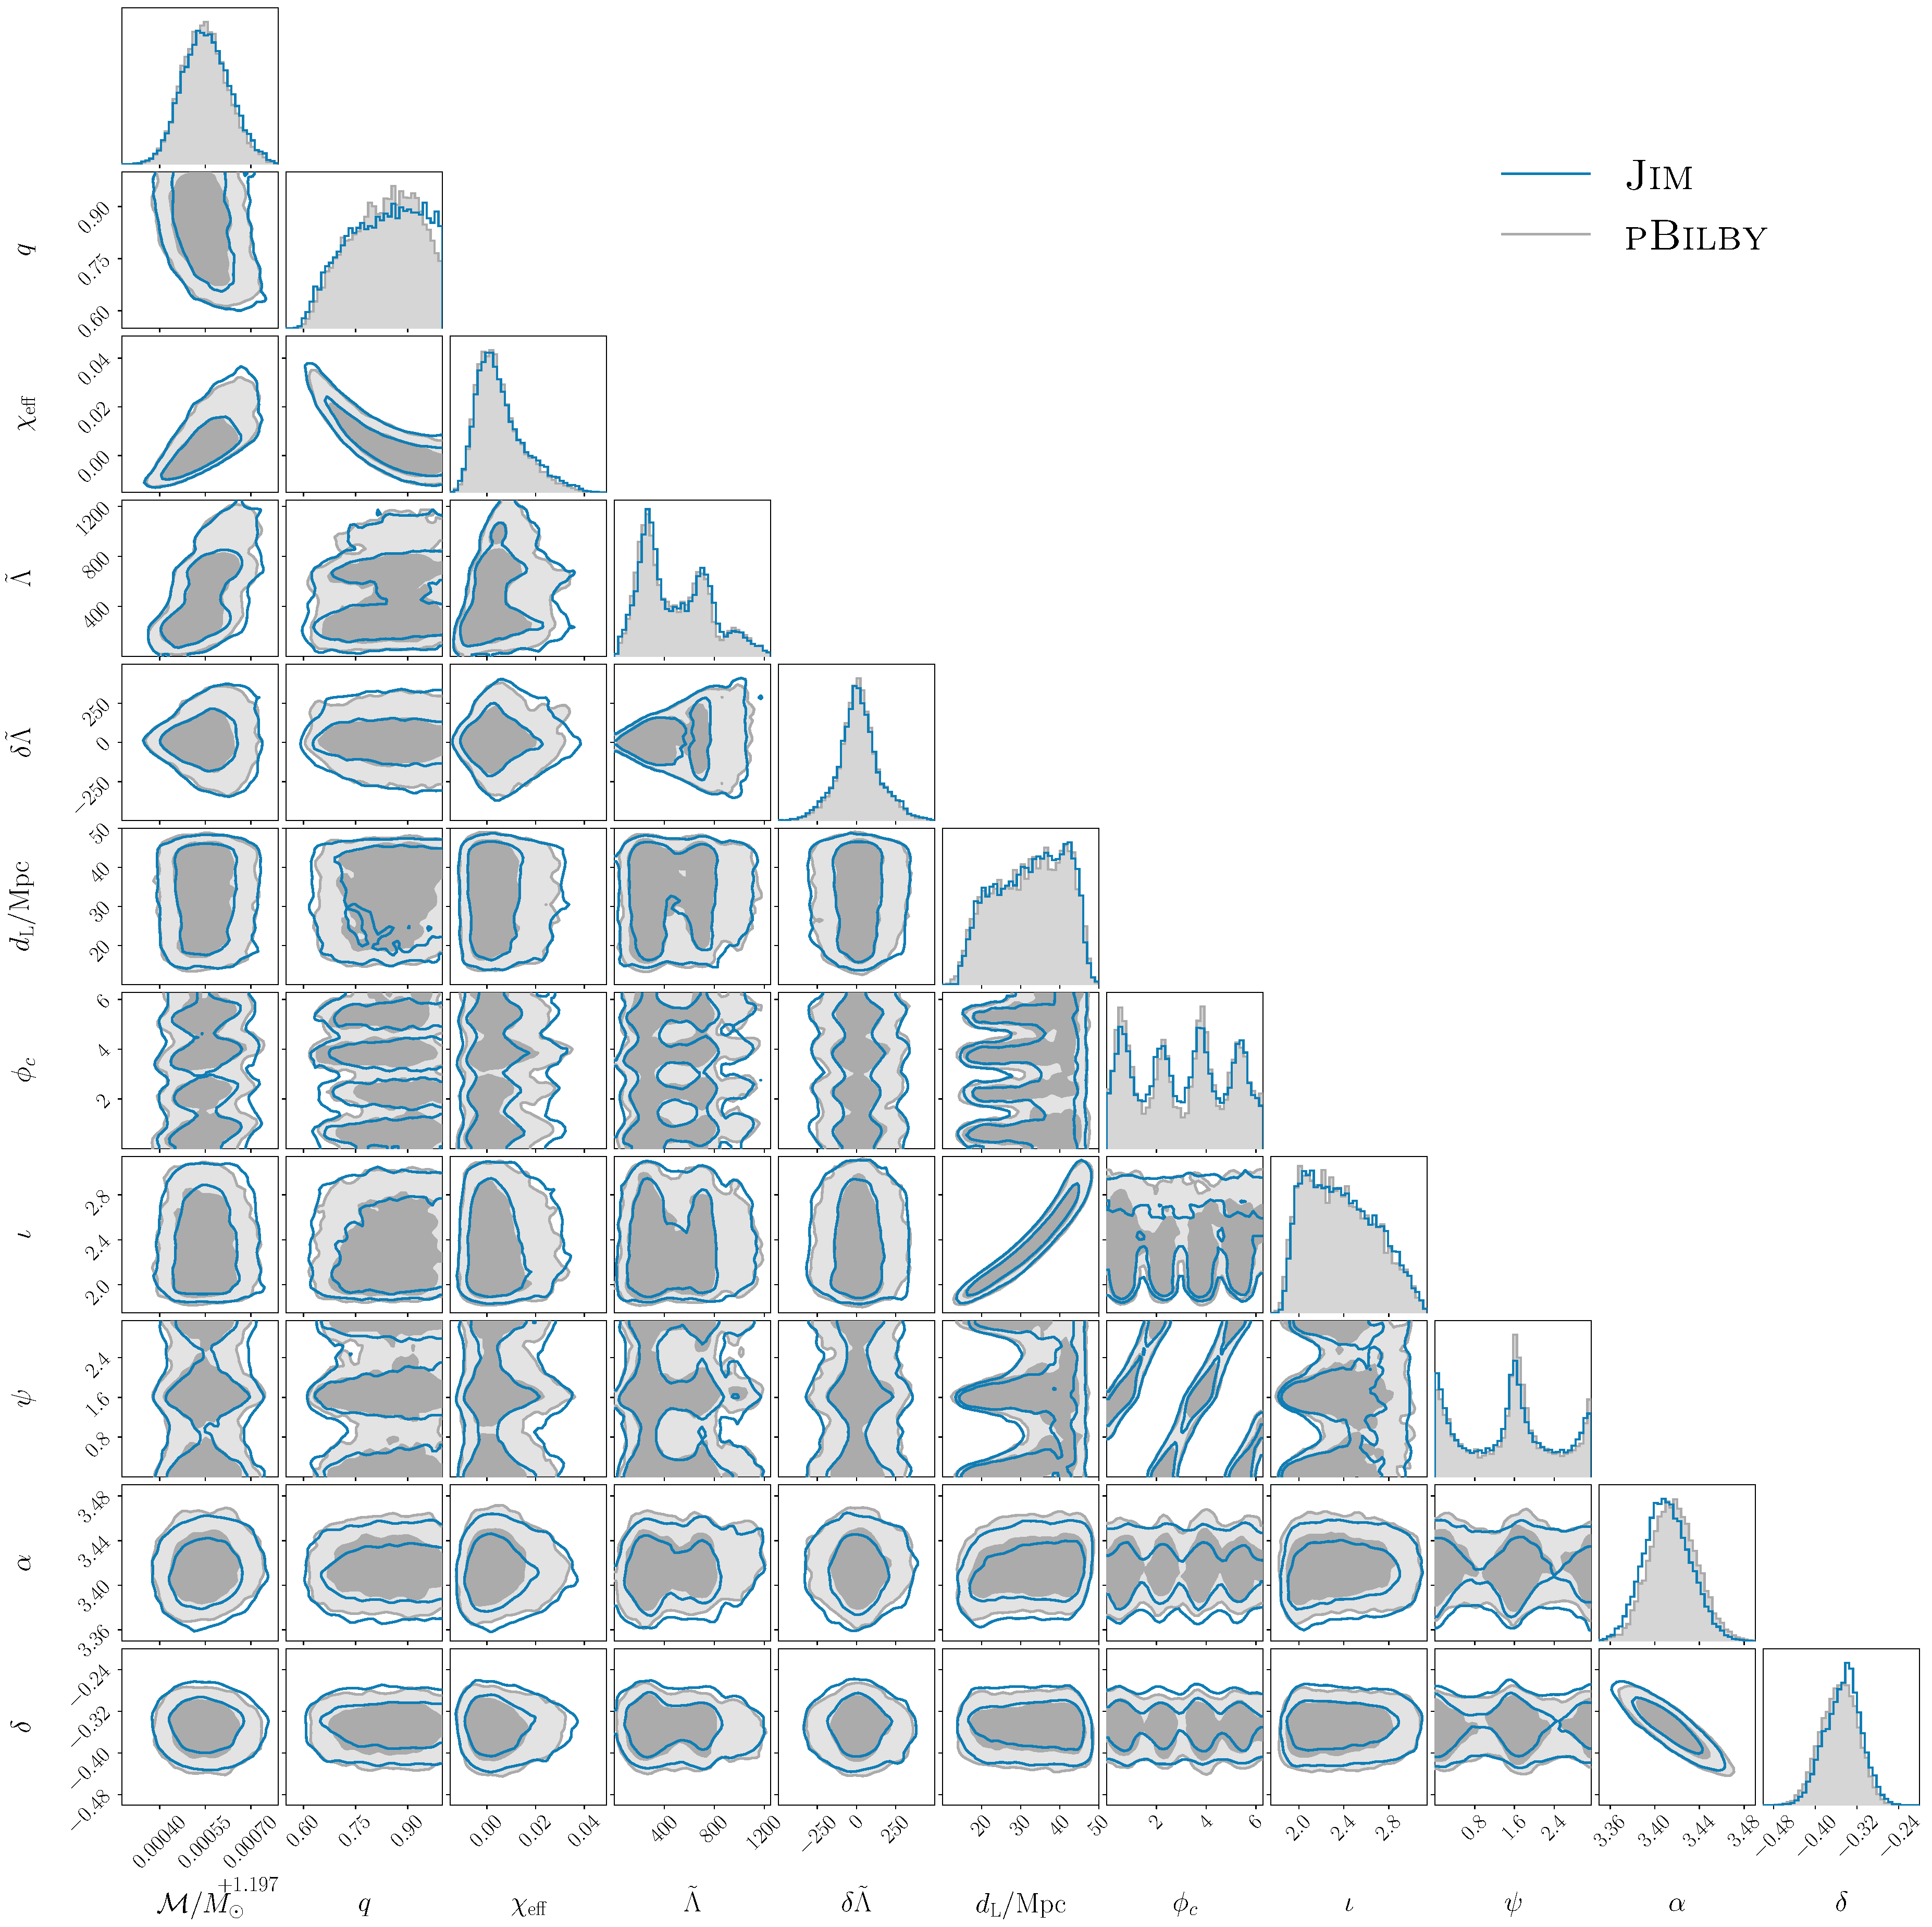
\includegraphics[scale = 0.132]{Figures/GW170817_TaylorF2.pdf}
%     \caption*{}
%     \end{figure}
%     \end{columns}
% \end{frame}

\begin{frame}{Environmental impact}
  
  \def\x{3mm}
  \def\y{1mm}

  \textsc{Jim} is \red{more environmentally friendly} than existing pipelines

  \vspace{\x}

  \begin{itemize}
    \item Energy consumption for all $204$ runs of paper
    
    \vspace{\x}

    \item Convert to number of trees to capture the emitted $\rm{CO}_2$ in a year.
  \end{itemize}
  
  \vspace{\y}

  \footnotesize
%   \begin{table}
%     \centering
%     \renewcommand{\arraystretch}{1.25}
%     \begin{tabular*}{0.95\linewidth}{@{\extracolsep{\fill}} l c r c r}
%       \hline\hline
% & & kWh & $\rm{CO}_2$ \footnotesize [$10^3$ kg] \normalsize & Trees${}^\dagger$ \\
%  \hline\hline
%  \textsc{Jim} & & $\phantom{00}33.78$ & $0.01$ & $0.55$ \\ \hline 
%  \textsc{pBilby} & & $3598.53$ & $1.18$ & $59.02$ \\ \hline 
%  \textsc{RB-\textsc{Bilby}} & & $90.78$ & $0.03$ & $1.49$ \\ \hline 
%  \multirow{2}{*}{\textsc{ROQ-Bilby}} & sampling & $32.00$ & $0.01$ & $0.52$ \\ 
%  & precompute${}^\ddagger$ & $5634.06$ & $1.85$ & $92.40$ \\
% \hline\hline
%     \end{tabular*}
%     \label{tab: environmental impact}
% \end{table}
\begin{table}
  \centering
  \renewcommand{\arraystretch}{1.5}
  \begin{tabular*}{0.75\linewidth}{@{\extracolsep{\fill}} l c r}
  \hline\hline
  Method & & Trees \\
  \hline\hline
  \textsc{Jim} & & $\phantom{000}0.55$ \\ \hline 
  \textsc{pBilby} & &  $59.02$ \\ \hline 
  \textsc{\textsc{RB-Bilby}} & & $1.49$ \\ \hline 
  \multirow{2}{*}{\textsc{ROQ-Bilby}} & sampling & $0.52$ \\ 
  & precompute${}^\ddagger$ & $0.44$ \\
  \hline\hline
  \end{tabular*}
  \label{tab: environmental impact}
\end{table}


% ${}^\dagger$Number of trees needed to capture the emitted $\rm{CO}_2$ in a year.

${}^\dagger$Estimated cost to build ROQ bases.
\normalsize
\end{frame}

\section{Conclusion}

\begin{frame}{Conclusion}

  \def\x{5mm}
  \def\y{3mm}
  \def\z{-4mm}

  \textsc{Jim}: a fast and environmentally friendly PE pipeline for GW signals
  
  \vspace{\y}

  \begin{itemize}
    % \item Enhance MCMC with
    % \begin{itemize}
    %   \vspace{\y}
    %   \item \textsc{jax},
    %   \vspace{\y}
    %   \item relative binning,
    %   \vspace{\y}
    %   \item gradient-based samplers, and
    %   \vspace{\y}
    %   \item normalizing flows
    % \end{itemize}
    
    
    % \vspace{\x}

    \item \texttt{TaylorF2} and \texttt{IMRPhenomD\_NRTidalv2} in \textsc{ripple}
    
    \vspace{\x}

    \item Parameter estimation of BNS in $15$ -- $30$ minutes sampling time without pretraining

    % \vspace{\x}

    % \item Science cases:
    % \begin{itemize}
    %   \vspace{\y}
    %   \item low-latency alerts,

    %   \vspace{\y}

    %   \item large-scale population studies, and future generation GW detectors
    % \end{itemize}
    
  \end{itemize}

  \vspace{\z}

  \begin{figure}
    \incfig[\textwidth]{jim_flowMC_ripple}
  \end{figure}
\end{frame}

\begin{frame}{References}

\nocite{*}

\printbibliography
    
\end{frame}

% ======== APPENDIX  ==========

\appendix

\begin{frame}[plain, noframenumbering]
\vfill
\centering
\textbf{APPENDIX}
\vfill
\end{frame}

\begin{frame}{Normalizing flow details}

  \def\x{3mm}

  \vspace{\x}

  \begin{itemize}
    \item Rational-quadratic neural spline flows
    
    \vspace{\x}
    
    \item 10 layers, 8 bins
    
    \vspace{\x}
    
    \item 128 neurons in hidden layers
    
    \vspace{\x}
    
    \item Adam optimizer, learning rate decayed (polynomial schedule)
    
    \vspace{\x}
    
    \item Deep learning library: \textsc{Equinox}
  \end{itemize}

  \vspace{\x}

  Loss function: KL divergence on sampled data
  \begin{equation*}
    \mathcal{L}(T) = - \frac1n \sum_{i=1}^n \log \hat{\rho}(x_i)
  \end{equation*}
  
\end{frame}


\begin{frame}{Stopping criterion}

  \def\x{2mm}

  We stop training the NF if we achieve a mean Metropolis-Hastings acceptance rate of $10\%$ ($20\%$) for real events (injections).

  \vspace{\x}

  Example: GW170817, \texttt{TaylorF2} with $20\%$: 

  \vspace{\x}

  \begin{figure}
    \centering
    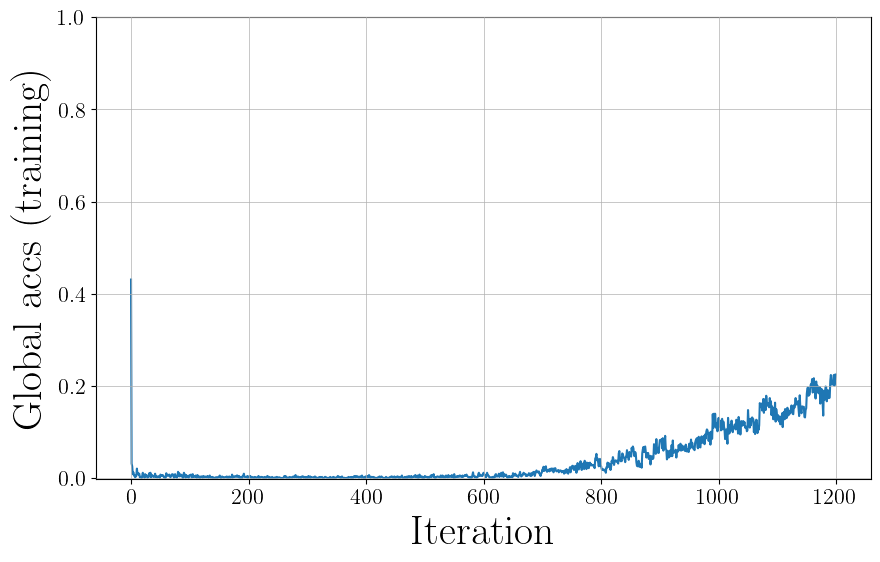
\includegraphics[width=0.75\textwidth]{Figures/global_accs_training.png}
  \end{figure}
\end{frame}

\begin{frame}{Validation -- Mismatch waveforms}

  Cross-check against \textsc{LALsuite}: mismatch histogram based on $10 \ 000$ waveforms, from uniform samples with following ranges:

  \footnotesize
  \begin{table}
    \centering
    \renewcommand{\arraystretch}{1.0}
    \begin{tabular}{l l} 
        \hline\hline
        Parameter & Range \\
        \hline
        Component masses & $[0.5M_{\odot}, 3M_{\odot}]$\\
        Component aligned spins & $[-0.05, 0.05]$\\
        Dimensionless tidal deformabilities &  $[0, 5000]$\\
        Inclination angle & $[0, \pi]$\\
        \hline\hline
    \end{tabular}
    \caption*{}
\end{table}
\normalsize

\vspace{-11.75mm}

  \begin{figure}
    \centering
    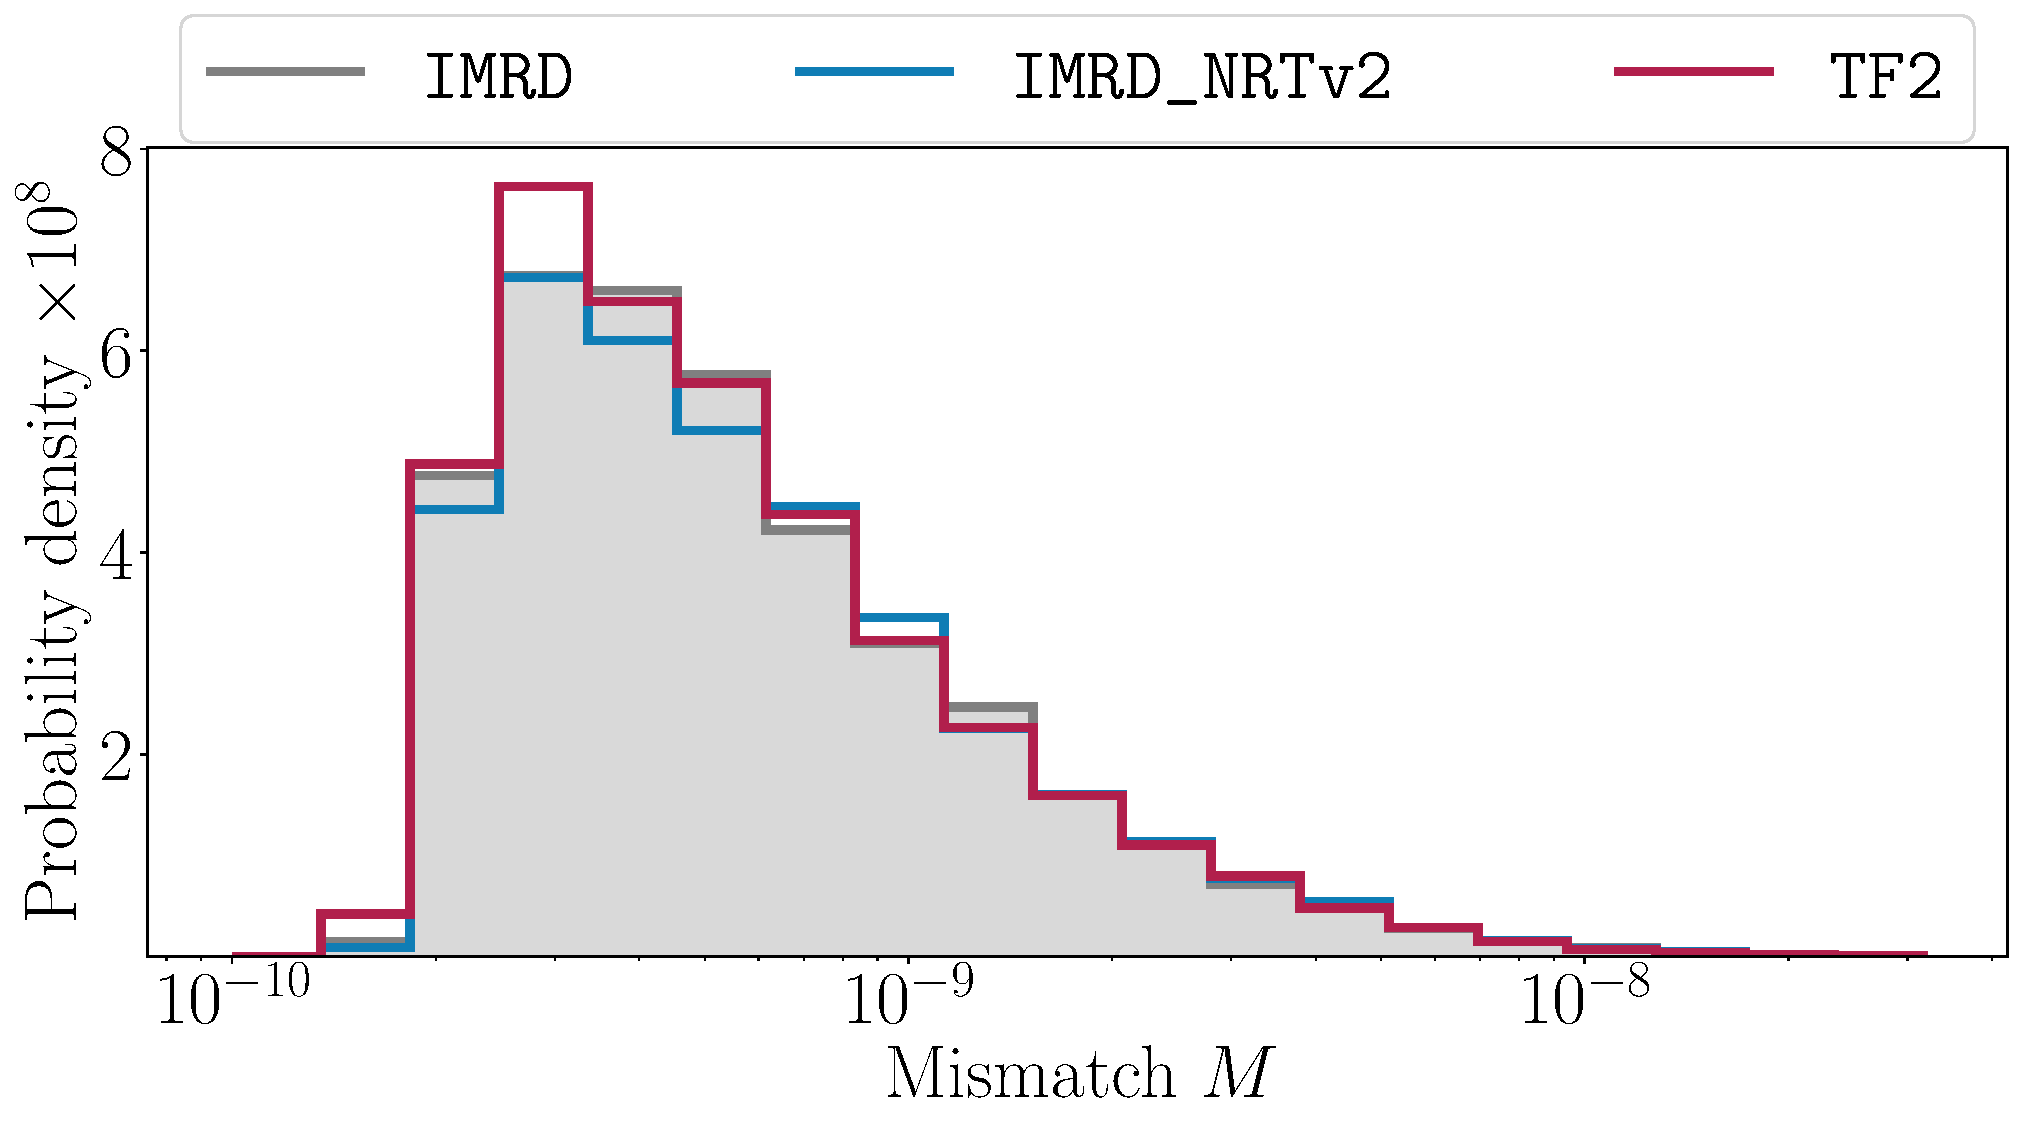
\includegraphics[width=0.7\textwidth]{Figures/mismatch_histogram.pdf}
    \caption*{}
  \end{figure}
  
\end{frame}


\begin{frame}{Validation -- p-p plot}
  
  \def\x{1mm}
  \def\y{3mm}

  We demonstrate the robustness of \textsc{Jim}:

  \begin{itemize}
    \item 100 GW events with HLV at design sensitivity and $T = 128$ s,
    
    \vspace{\x}

    \item \texttt{NRTv2}: reference waveform relative binning without taper,
    
    \vspace{\x}
    
    \item Priors: Table~\ref{tab:parameter_priors}.
  \end{itemize}


  \begin{columns}
    \column{0.49\textwidth}
    \begin{figure}
      \centering
      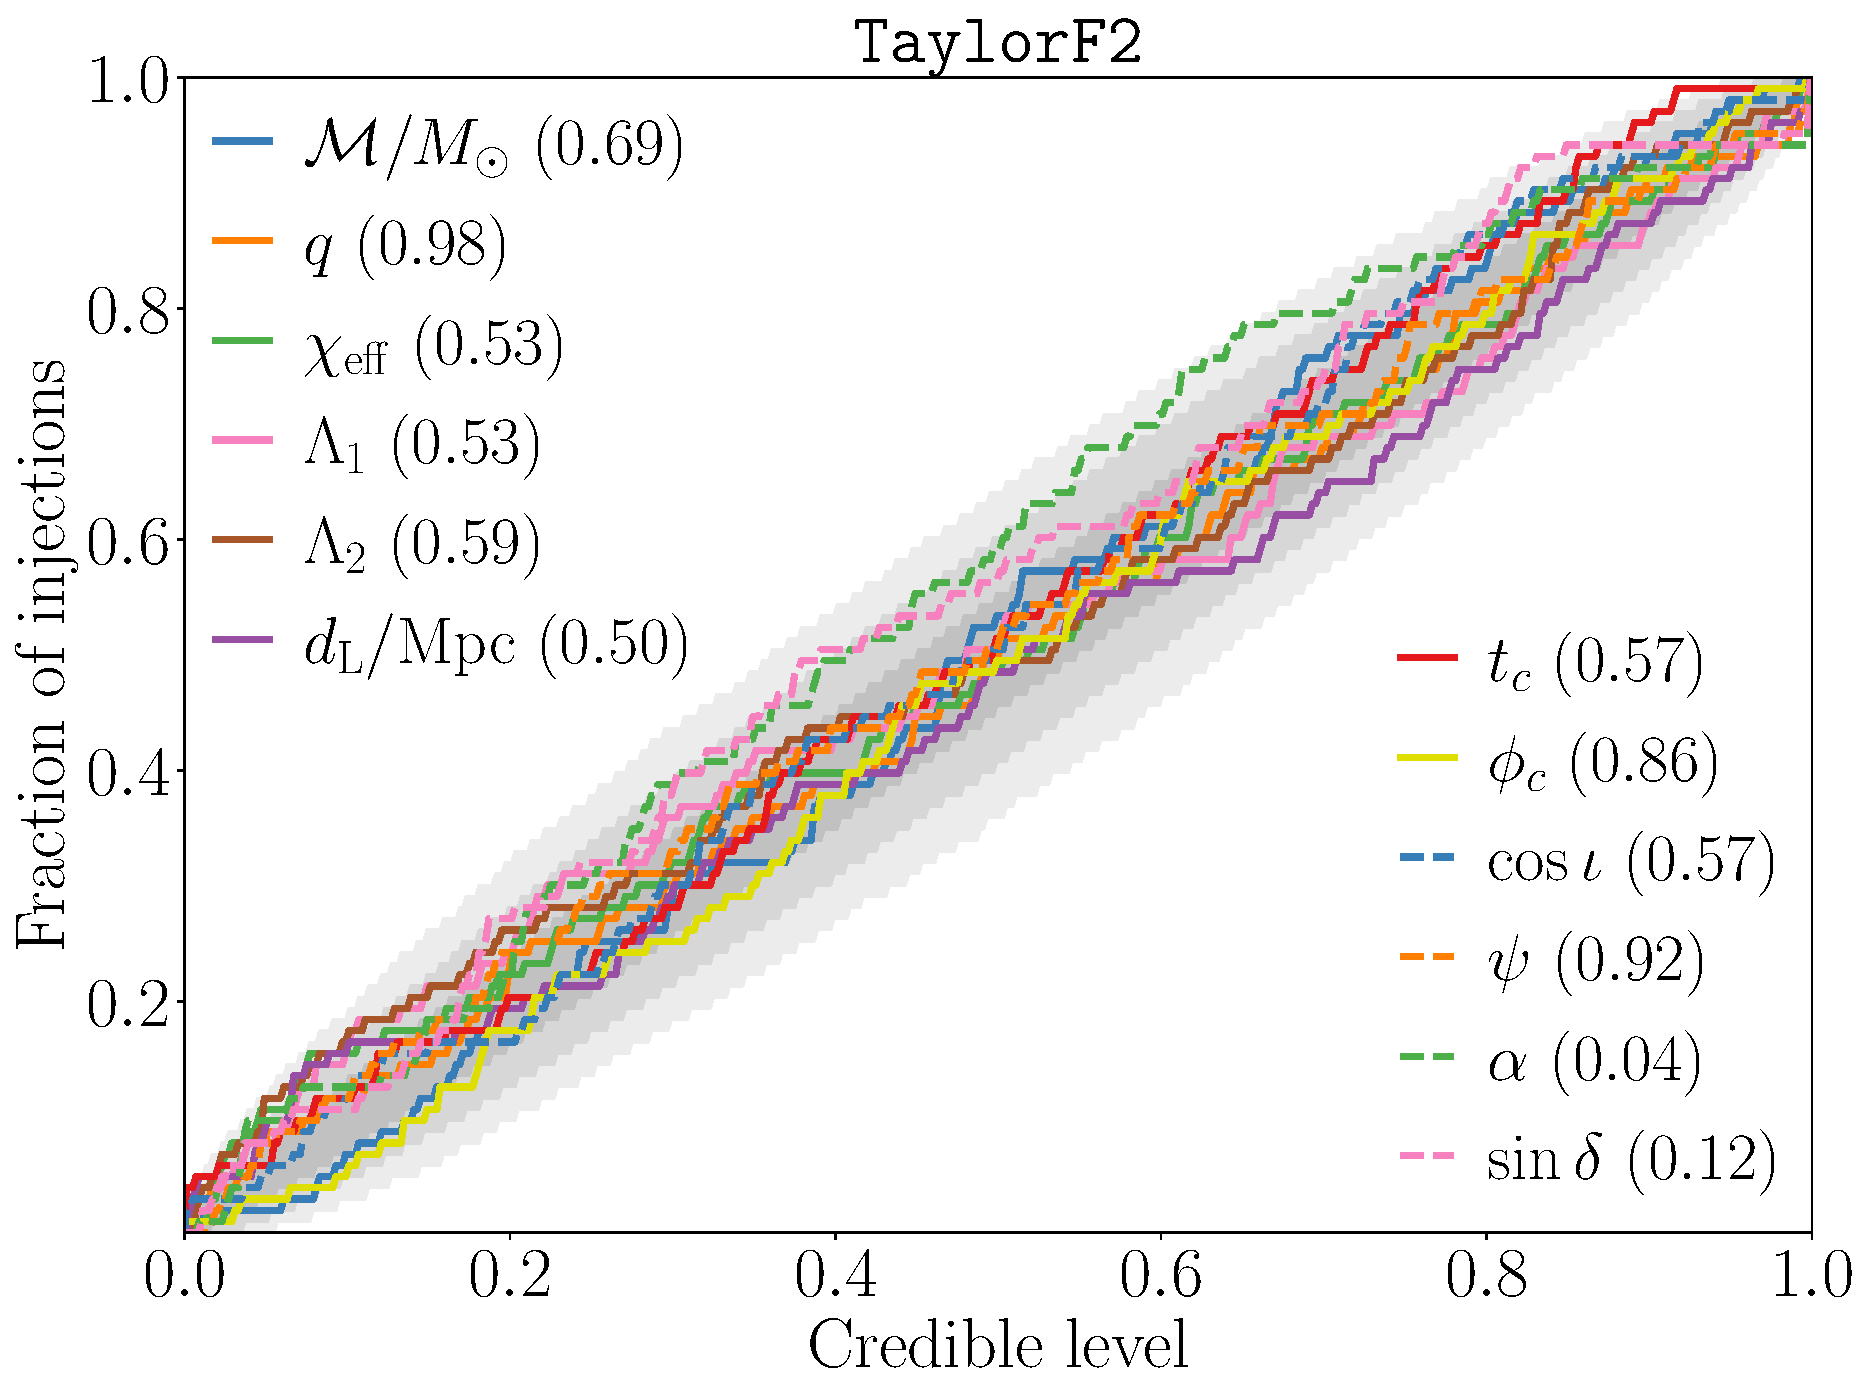
\includegraphics[width=\linewidth]{Figures/pp_plot_TF2.pdf}
    \end{figure}
    \column{0.49\textwidth}
    \begin{figure}
      \centering
      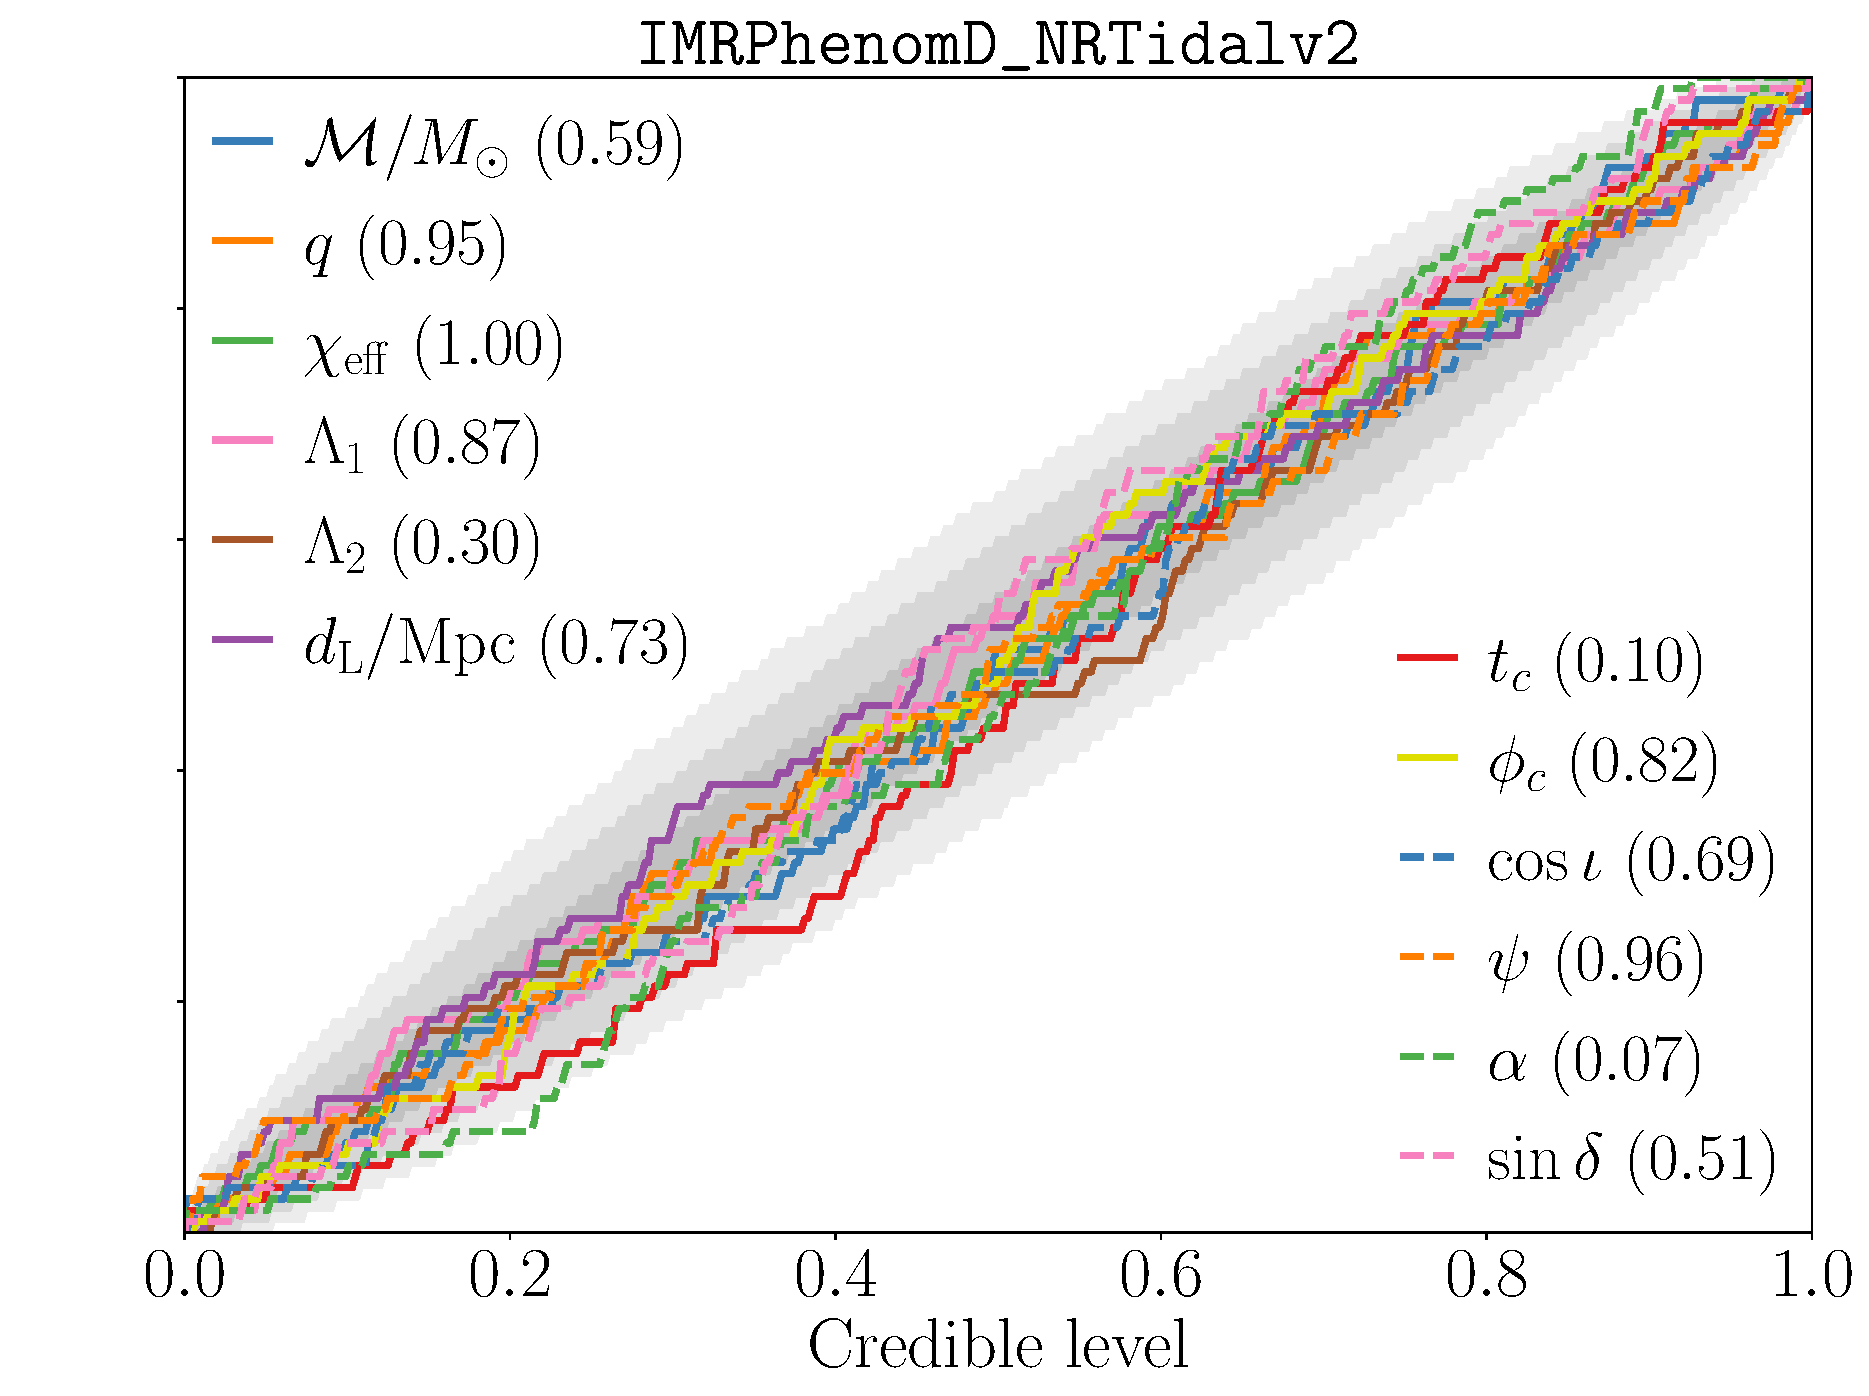
\includegraphics[width=\linewidth]{Figures/pp_plot_NRTv2.pdf}
    \end{figure}
  \end{columns}
\end{frame}

\begin{frame}{Priors}
  
  \begin{table}
    \caption{Prior ranges used in our analyses. All priors are uniform priors with the specified range.}
    \label{tab:parameter_priors}
    \renewcommand{\arraystretch}{1}
    % \begin{tabular}{\textwidth}{@{\extracolsep{\fill}} l l l l l}
      \begin{tabular}{l l l l l}
    \hline \hline
    Parameter  & Injection & GW170817 & GW190425 \\ \hline
    $\mathcal{M}$ $[M_\odot]$ & $[0.88, 2.61]$ & $[1.18, 1.21]$ & $[1.485, 1.490]$ \\
    $q$ & $[0.5, 1]$ & $[0.125, 1]$ & $[0.125, 1]$ \\ 
    $\chi_i$ & $[-0.05, 0.05]$ & $[-0.05, 0.05]$ & $[-0.05, 0.05]$ \\
    $\Lambda_i$ & $[0, 5000]$ & $[0, 5000]$ & $[0, 5000]$ \\
    $d_L$ $[\rm{Mpc}]$ & $[30, 300]$ & $[1, 75]$ & $[1, 500]$ \\
    $t_c$ $[\rm{s}]$ & $[-0.1, 0.1]$ & $[-0.1, 0.1]$ & $[-0.1, 0.1]$ \\
    $\phi_c$ & $[0, 2\pi]$ & $[0, 2\pi]$ & $[0, 2\pi]$ \\
    $\cos \iota$ & $[-1, 1]$ & $[-1, 1]$ & $[-1, 1]$ \\
    $\psi$ & $[0, \pi]$ & $[0, \pi]$ & $[0, \pi]$ \\
    $\alpha$ & $[0, 2\pi]$ & $[0, 2\pi]$ & $[0, 2\pi]$ \\
    $\sin \delta$ & $[-1, 1]$ & $[-1, 1]$ & $[-1, 1]$ \\
    \hline \hline
    \end{tabular}
\end{table}
\end{frame}


\begin{frame}{GW170817 \& GW190425: Jensen-Shannon divergences}

  \def\x{-1mm}
  
  \vspace{\x}

  \footnotesize

  \begin{table}
    \centering
    \def\arraystretch{1}
    \caption{Jensen-Shannon divergences (in bits) between the marginal posterior obtained for GW170817 and GW190425 using \texttt{TaylorF2} and \texttt{IMRPhenomD\_NRTidalv2} with \textsc{Jim} and \textsc{pBilby}, with the highest value of each comparison in bold. The divergences are bound between $[0, 1]$.}
    \begin{tabular*}{\textwidth}{@{\extracolsep{\fill}} l  c  c  c  c }

      \hline\hline
& \multicolumn{2}{ c }{GW170817} & \multicolumn{2}{ c }{GW190425} \\
Parameter & \texttt{TF2} & \texttt{NRTv2} & \texttt{TF2} & \texttt{NRTv2} \\ \hline
      
$\mathcal{M}$ & $0.001725$ & $0.000516$ & $0.003557$ & $0.002461$ \\
$q$ & $0.005212$ & $0.007894$ & $0.004837$ & $0.002960$ \\
$\chi_1$ & $0.005633$ & $0.004301$ & $0.002794$ & $0.004825$ \\
$\chi_2$ & $0.003030$ & $0.002671$ & $0.002416$ & $0.003041$ \\
$\Lambda_1$ & $0.001062$ & $0.002208$ & $0.008556$ & $0.000783$ \\
$\Lambda_2$ & $0.000559$ & $0.002186$ & $0.005808$ & $0.003576$ \\
$d_L$ & $0.001544$ & $\bm{0.01847}$ & $0.001273$ & $0.002878$ \\
$\phi_c$ & $0.003500$ & $0.010714$ & $0.003338$ & $0.006126$ \\
$\cos \iota$ & $0.001615$ & $0.012851$ & $0.006400$ & $0.005279$ \\
$\psi$ & $0.004048$ & $0.011036$ & $0.001516$ & $0.003730$ \\
$\alpha$ & $\bm{0.014008}$ & $0.001258$ & $\bm{0.009822}$ & $\bm{0.012291}$ \\
$\sin \delta$ & $0.009570$ & $0.001761$ & $0.008934$ & $0.009228$ \\
\hline\hline
    \end{tabular*}
    \label{tab: JS divergences events}
\end{table}
\normalsize
\end{frame}

\begin{frame}{GW170817 with \texttt{TaylorF2}}
  \vspace{-4.5mm}
  \begin{figure}

    \begin{minipage}[c]{0.2\textwidth}
    \caption{}\label{fig: GW170817 TaylorF2}
    \end{minipage}\hfill
    \begin{minipage}[c]{0.8\textwidth}
    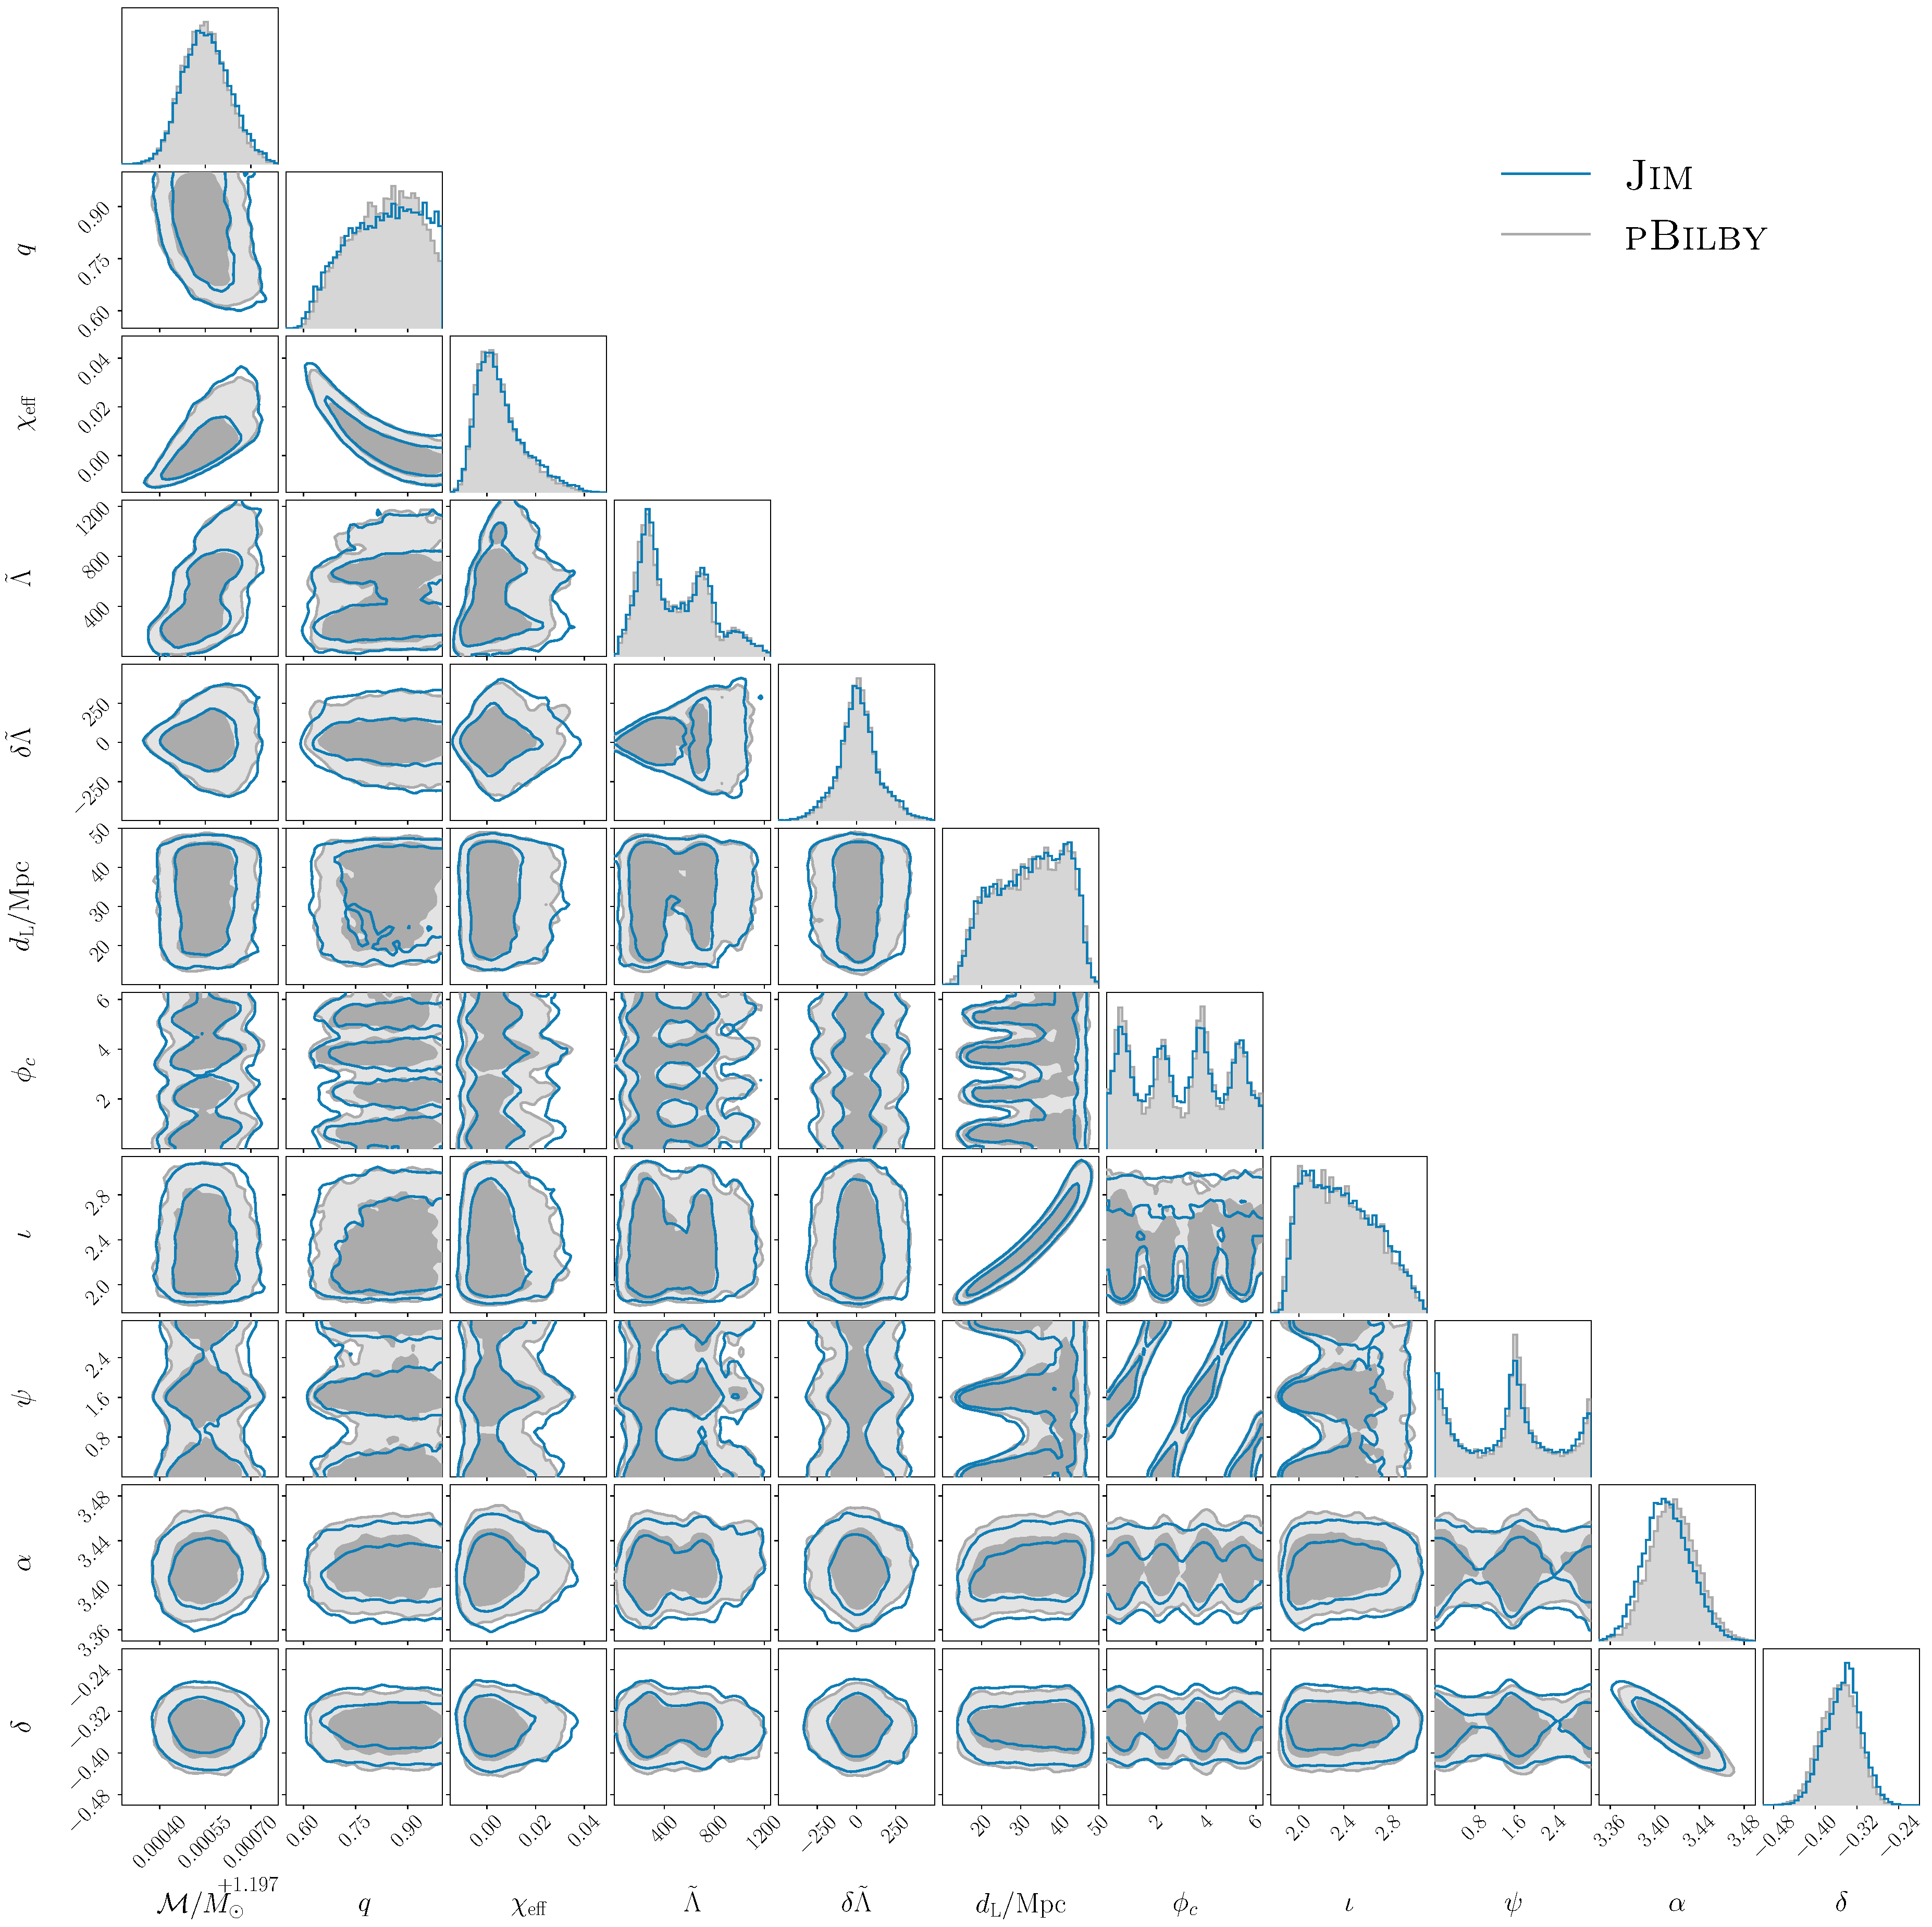
\includegraphics[scale = 0.132]{Figures/GW170817_TaylorF2.pdf}
    \end{minipage}
    
  \end{figure}
\end{frame}

\begin{frame}{GW170817 with \texttt{IMRPhenomD\_NRTidalv2}}
  \vspace{-4.5mm}
  \begin{figure}
  
  \begin{minipage}[c]{0.2\textwidth}
    \caption{}\label{fig: GW170817 NRTidalv2}
    \end{minipage}\hfill
    \begin{minipage}[c]{0.8\textwidth}
    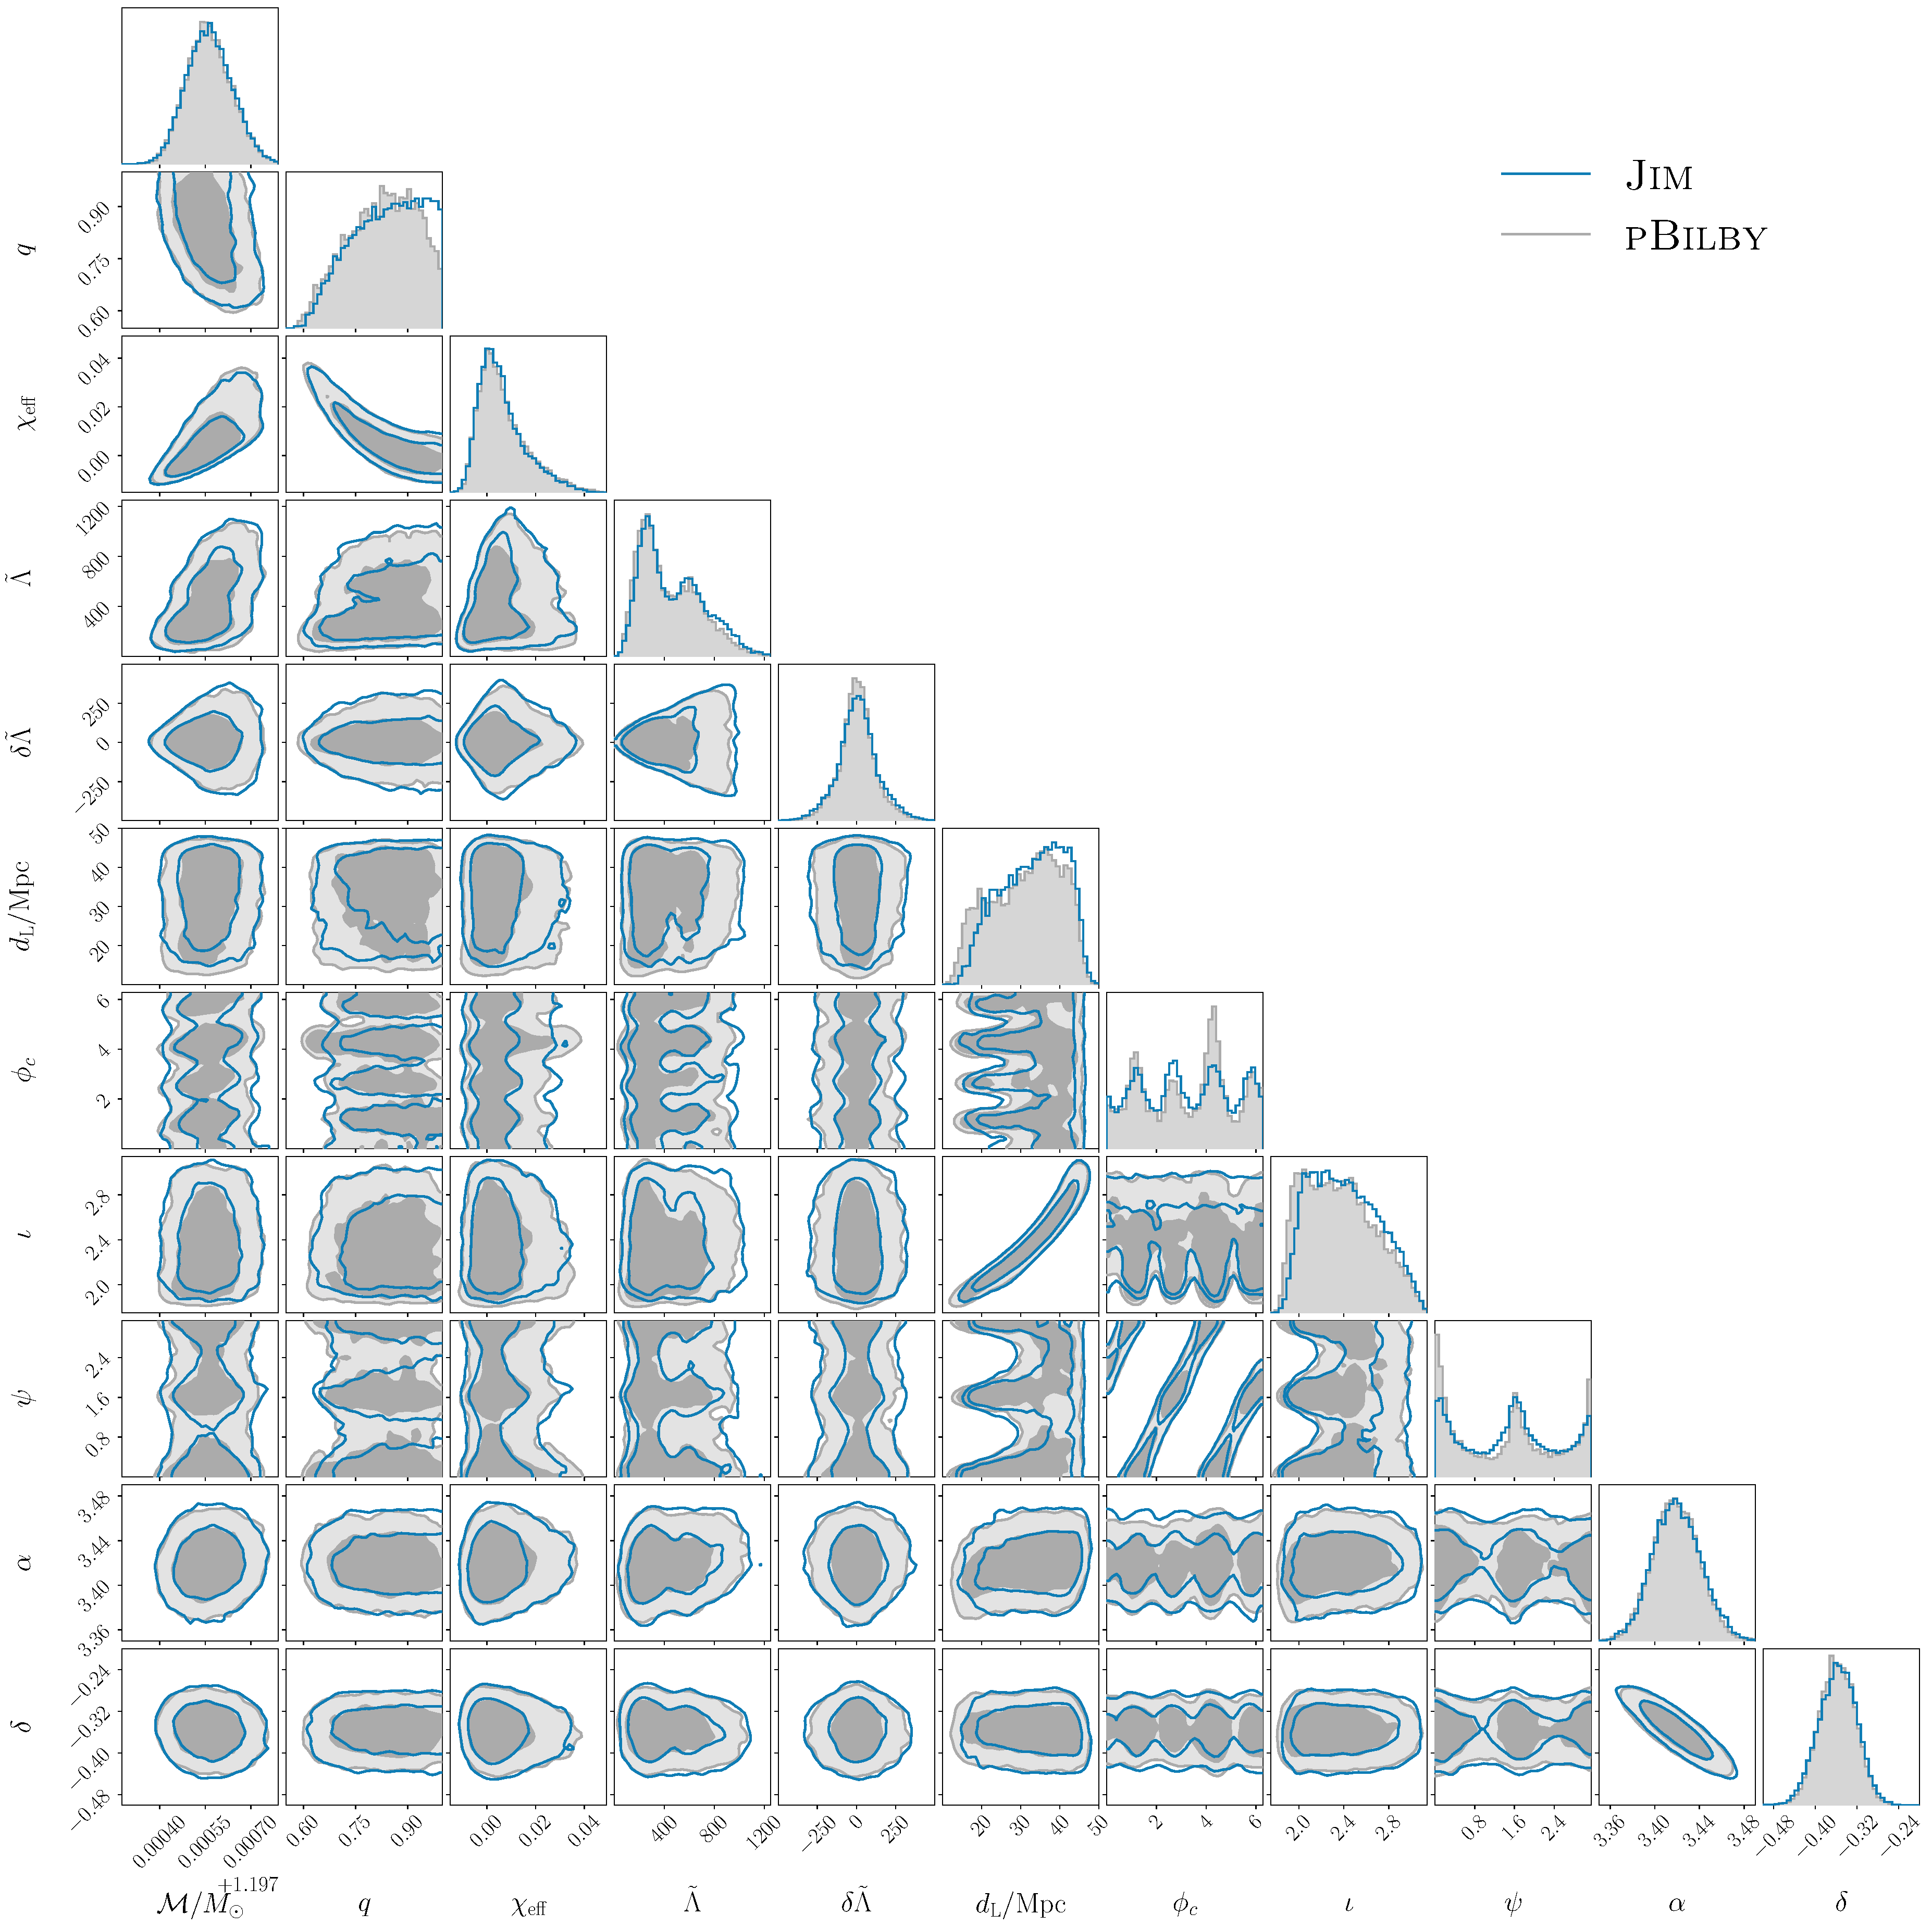
\includegraphics[scale = 0.132]{Figures/GW170817_NRTidalv2.pdf}
    \end{minipage}
  \end{figure}
\end{frame}


\begin{frame}{GW190425 with \texttt{TaylorF2}}
  \vspace{-4.5mm}
  \begin{figure}
  
  \begin{minipage}[c]{0.2\textwidth}
    \caption{}\label{fig: GW190425 TaylorF2}
    \end{minipage}\hfill
    \begin{minipage}[c]{0.8\textwidth}
    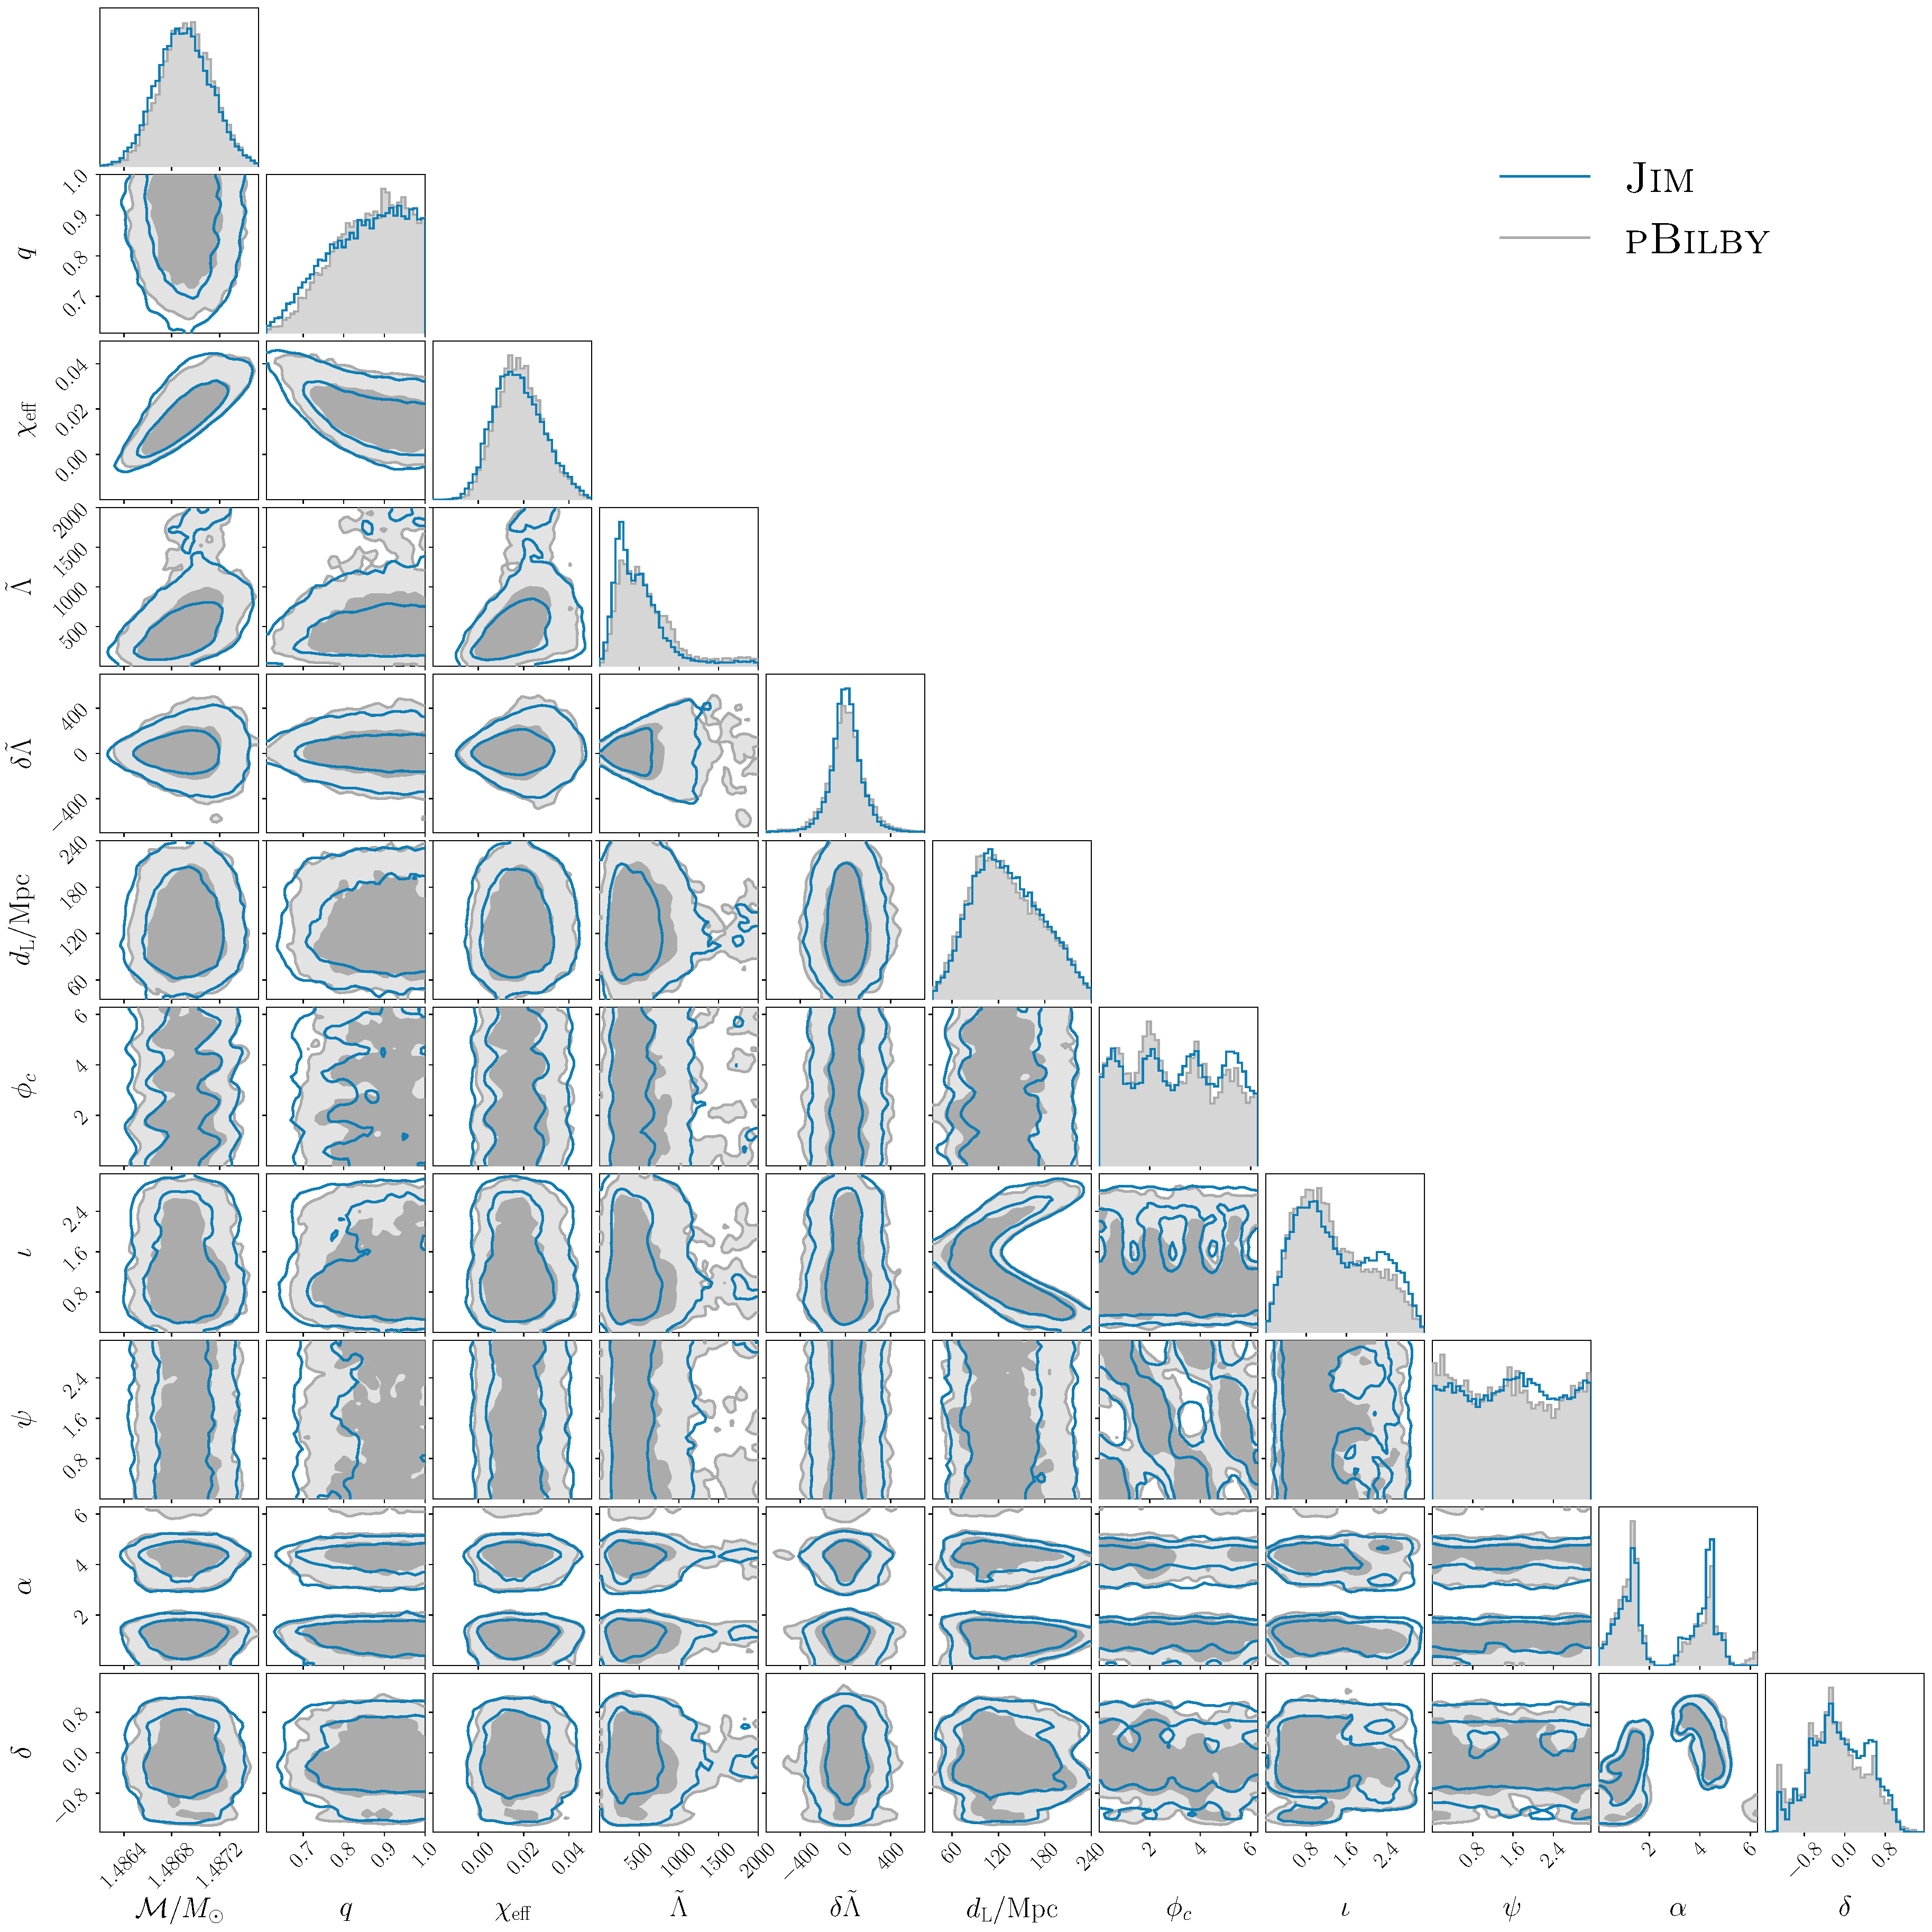
\includegraphics[scale = 0.132]{Figures/GW190425_TaylorF2.pdf}
    \end{minipage}
  \end{figure}
\end{frame}

\begin{frame}{GW190425 with \texttt{IMRPhenomD\_NRTidalv2}}
  \vspace{-4.5mm}
  \begin{figure}
  \begin{minipage}[c]{0.2\textwidth}
    \caption{}\label{fig: GW190425 NRTidalv2}
    \end{minipage}\hfill
    \begin{minipage}[c]{0.8\textwidth}
    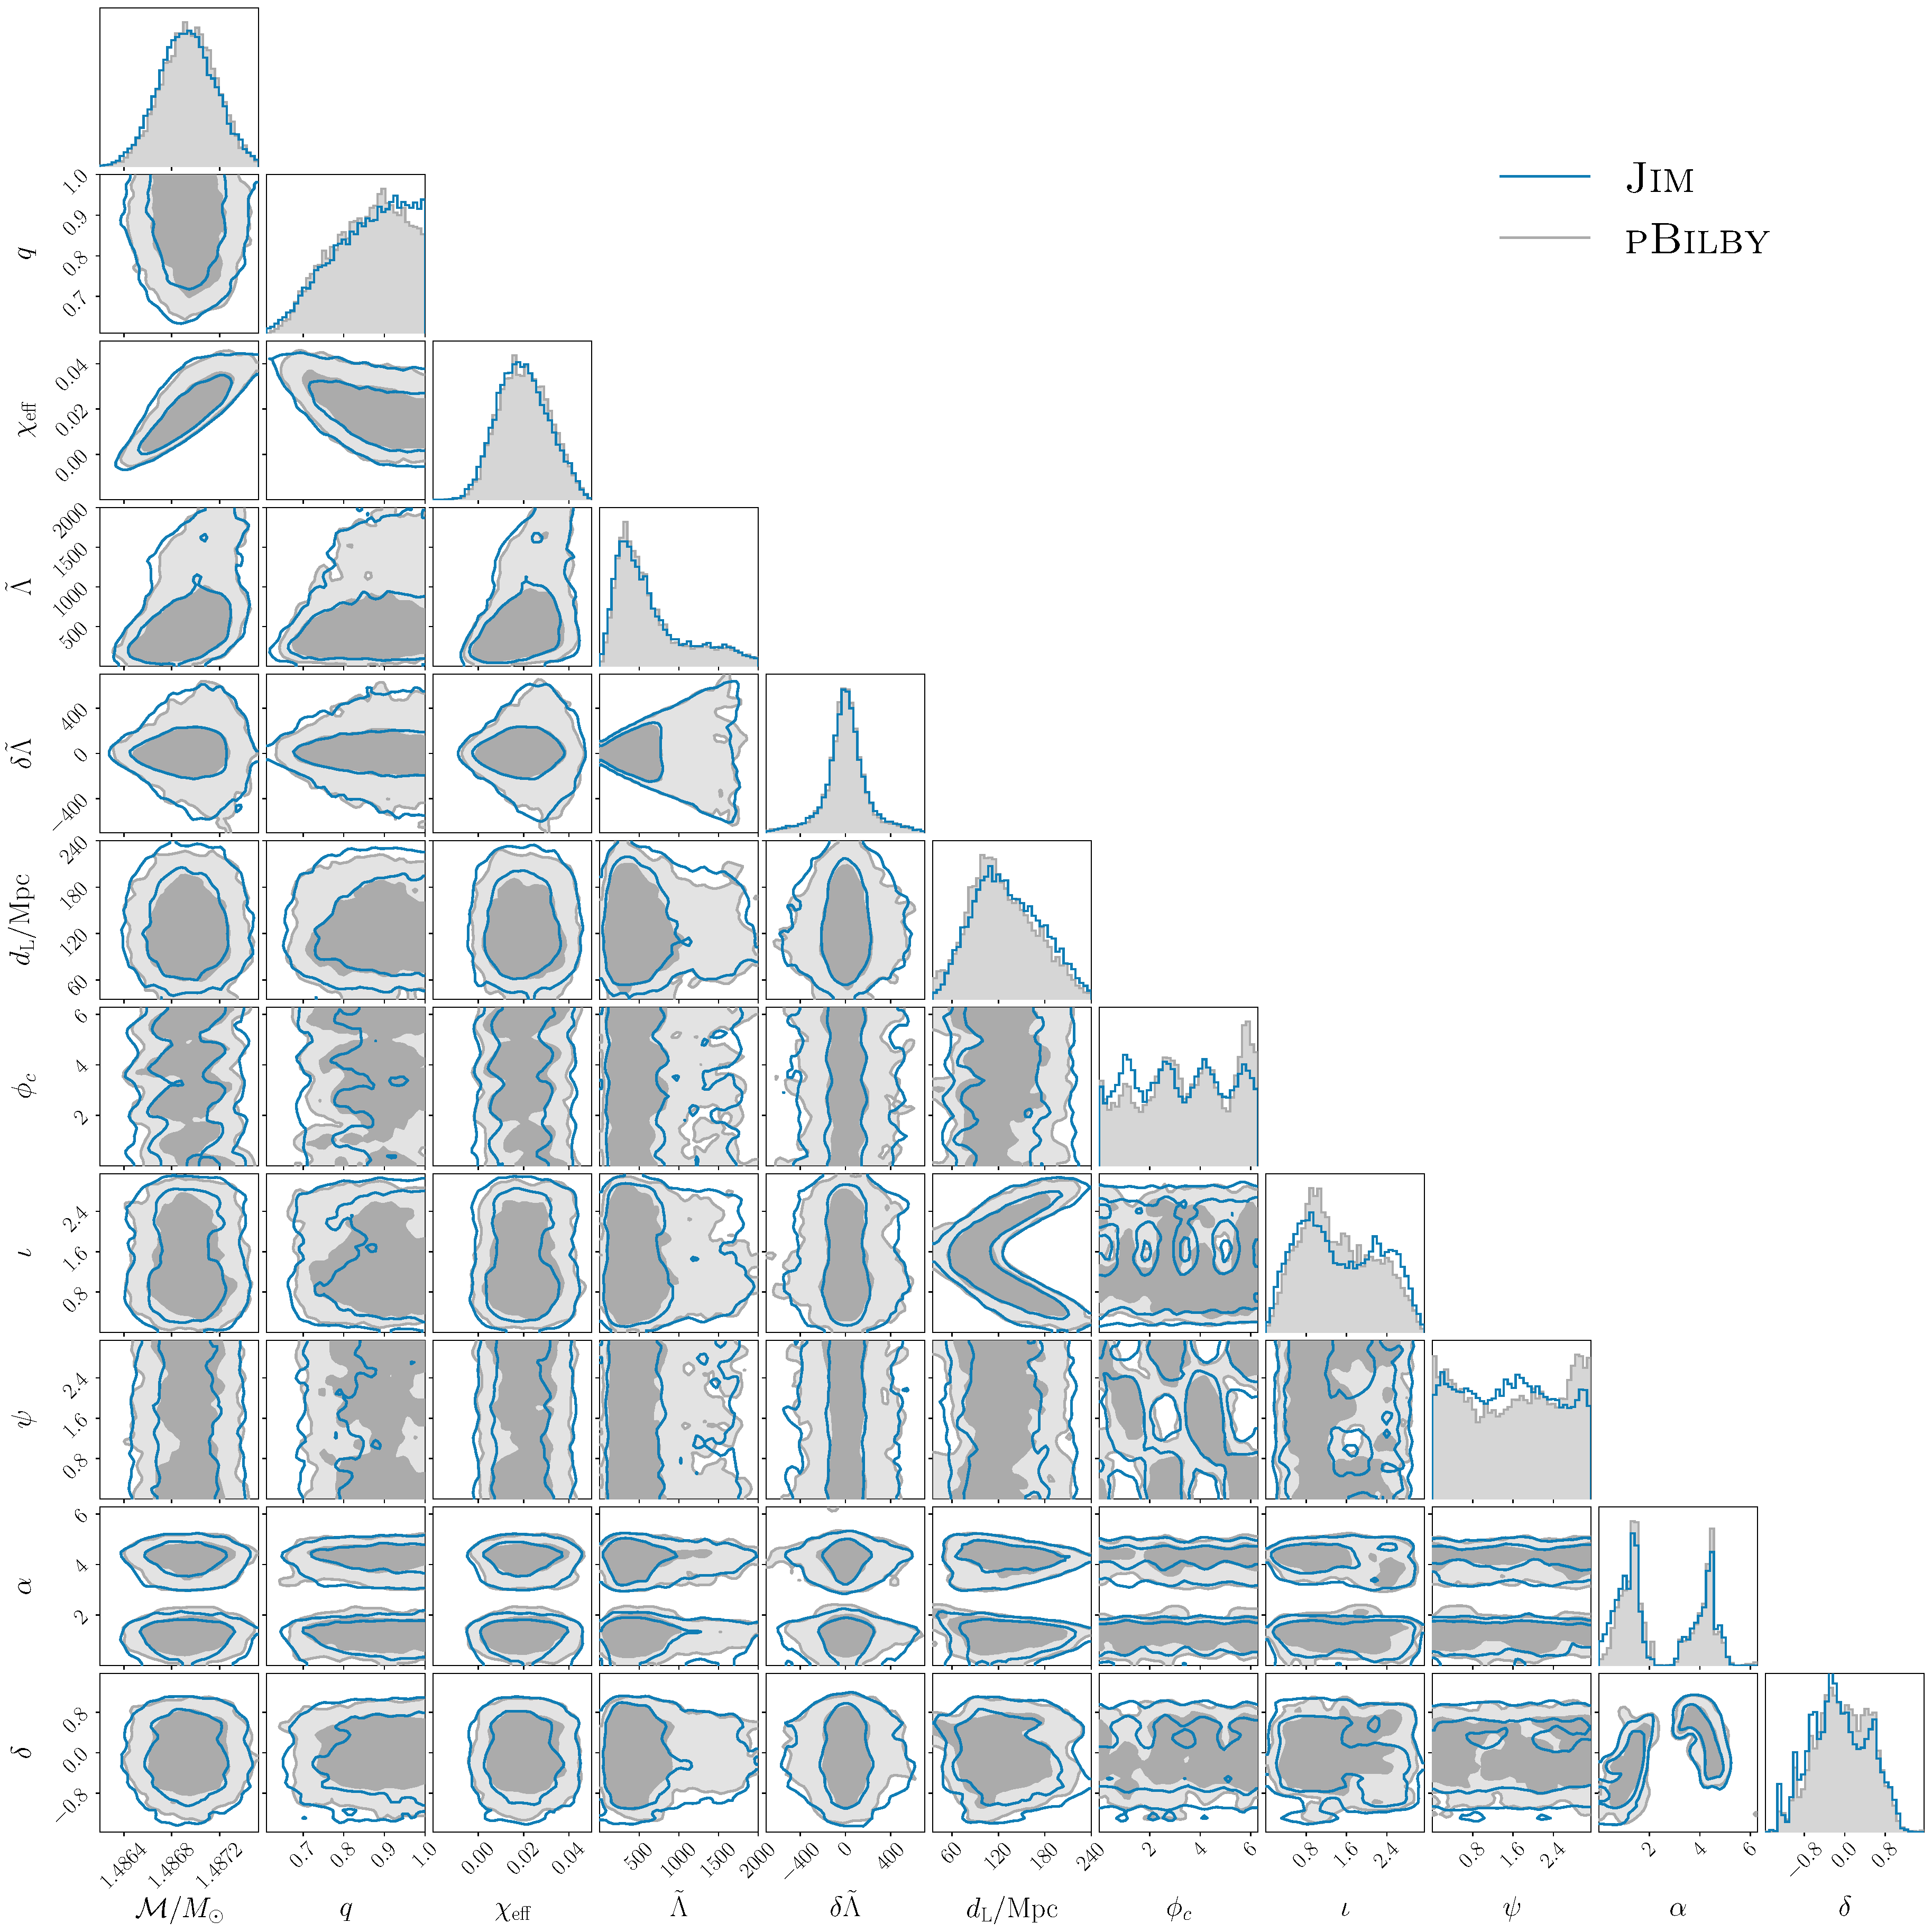
\includegraphics[scale = 0.132]{Figures/GW190425_NRTidalv2.pdf}
  \end{minipage}  
  \end{figure}
  
\end{frame}



\end{document}

